\section{Results}

\figref{paramLGM} shows the counts from the left GM tube over the full range of parameter space explored, with the electron gun both on and off; \figref{paramRGM} shows the same 
data for the right GM tube. 

\begin{figure}[h!]
    \centering
    \subcaptionbox{Count rate from left GM tube as a function of anode voltage and acetone pressure. Electron gun off}[0.49\linewidth]{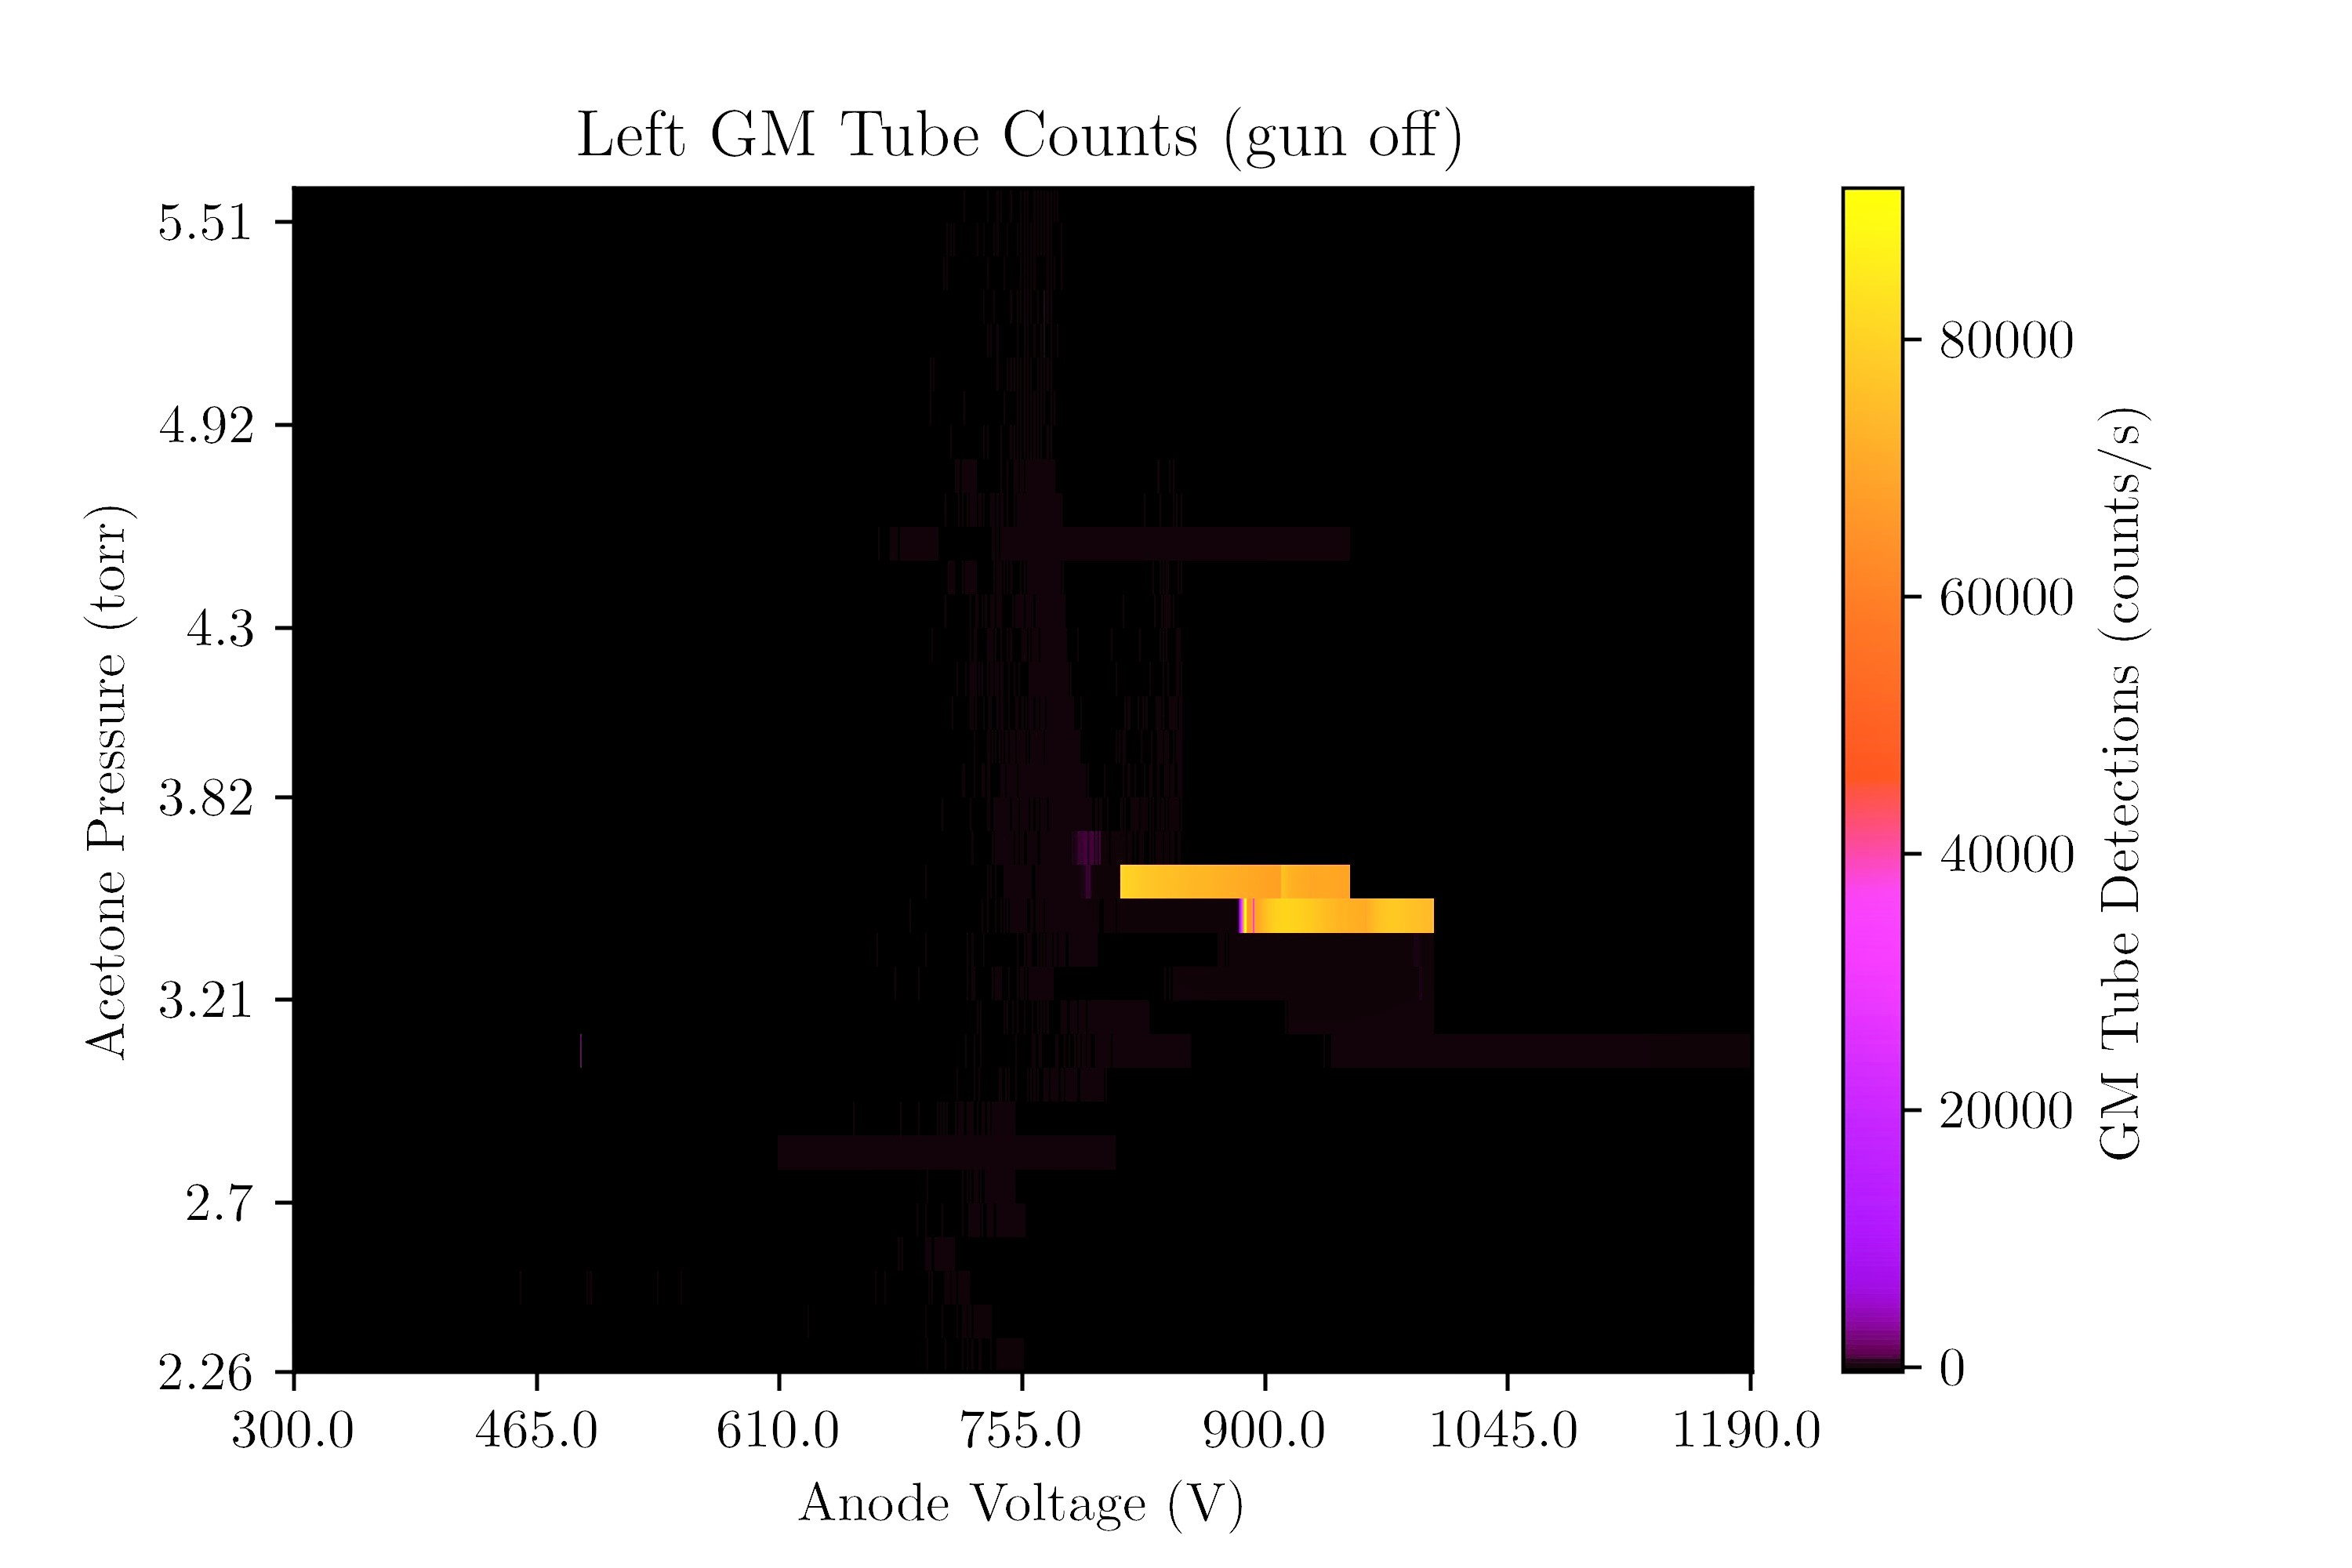
\includegraphics[scale=0.65]{Figs/LGMGunOff.jpg}}
    \subcaptionbox{Count rate from left GM tube as a function of anode voltage and acetone pressure. Electron gun on}[0.49\linewidth]{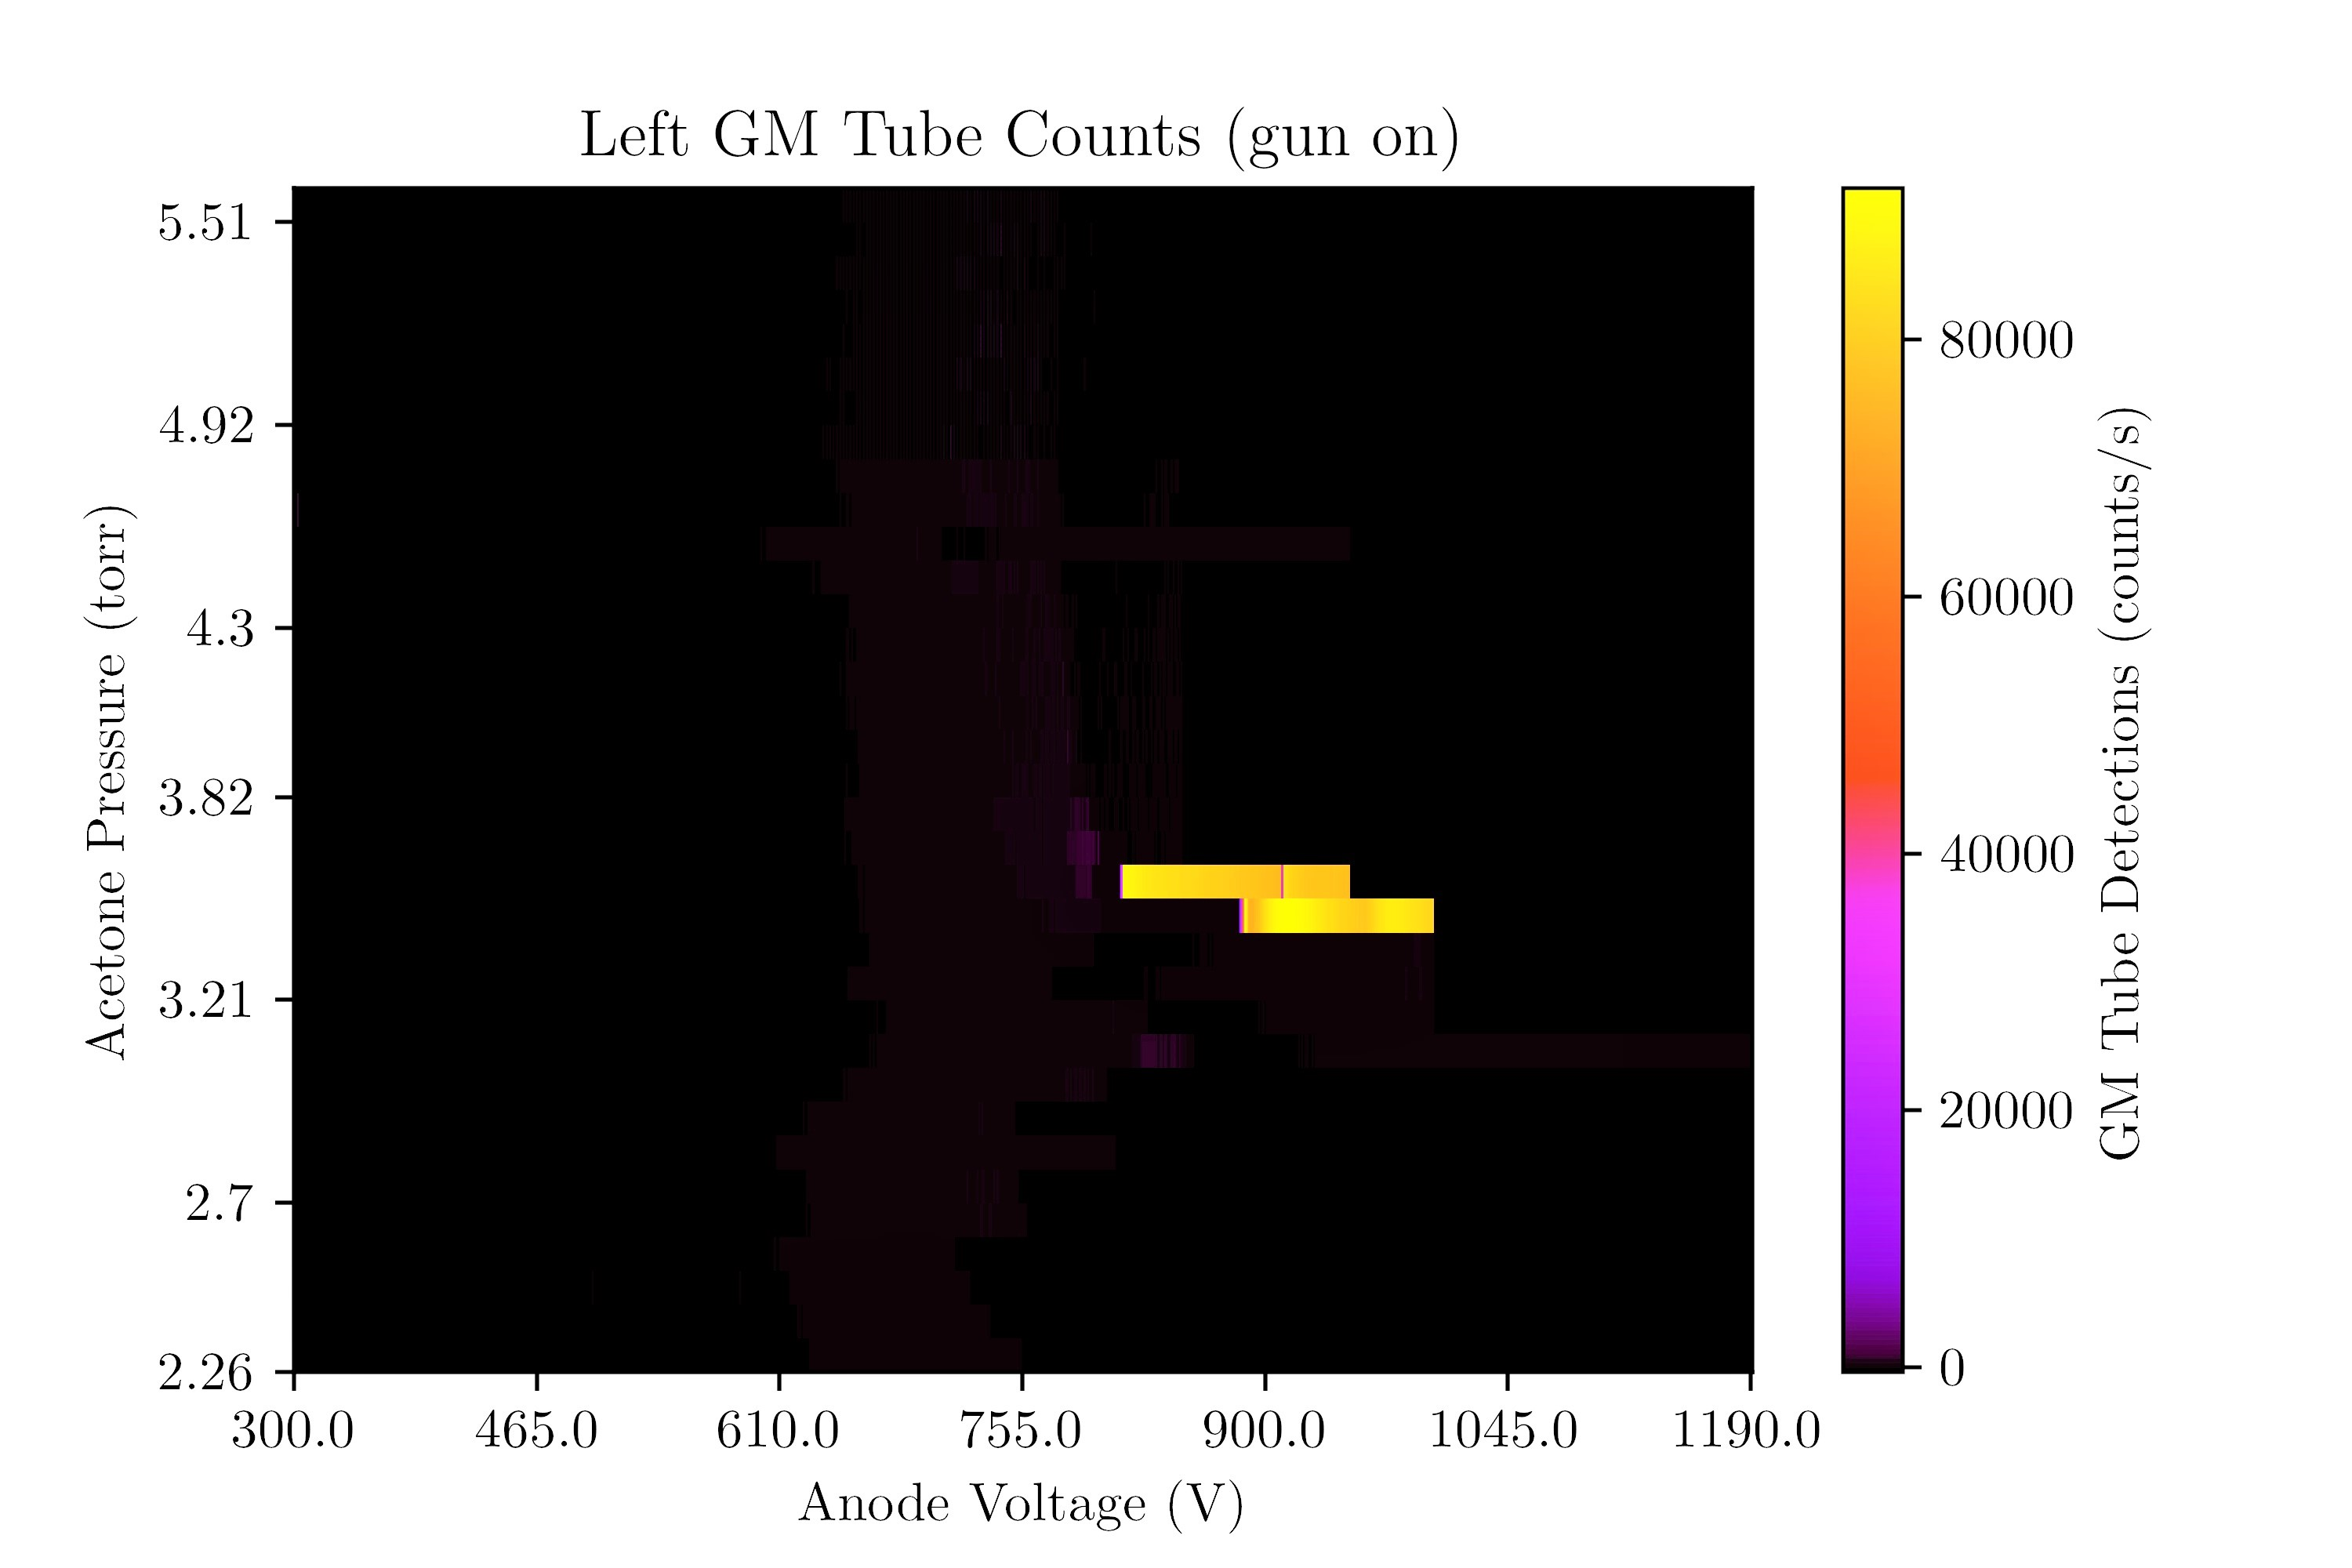
\includegraphics[scale=0.65]{Figs/LGMGunOn.jpg}}
    \caption{Performance of left GM tube over entire parameter space of pressures and voltages}
    \label{fig:paramLGM}
\end{figure}

\begin{figure}[h!]
    \centering
    \subcaptionbox{Count rate from right GM tube as a function of anode voltage and acetone pressure. Electron gun off}[0.49\linewidth]{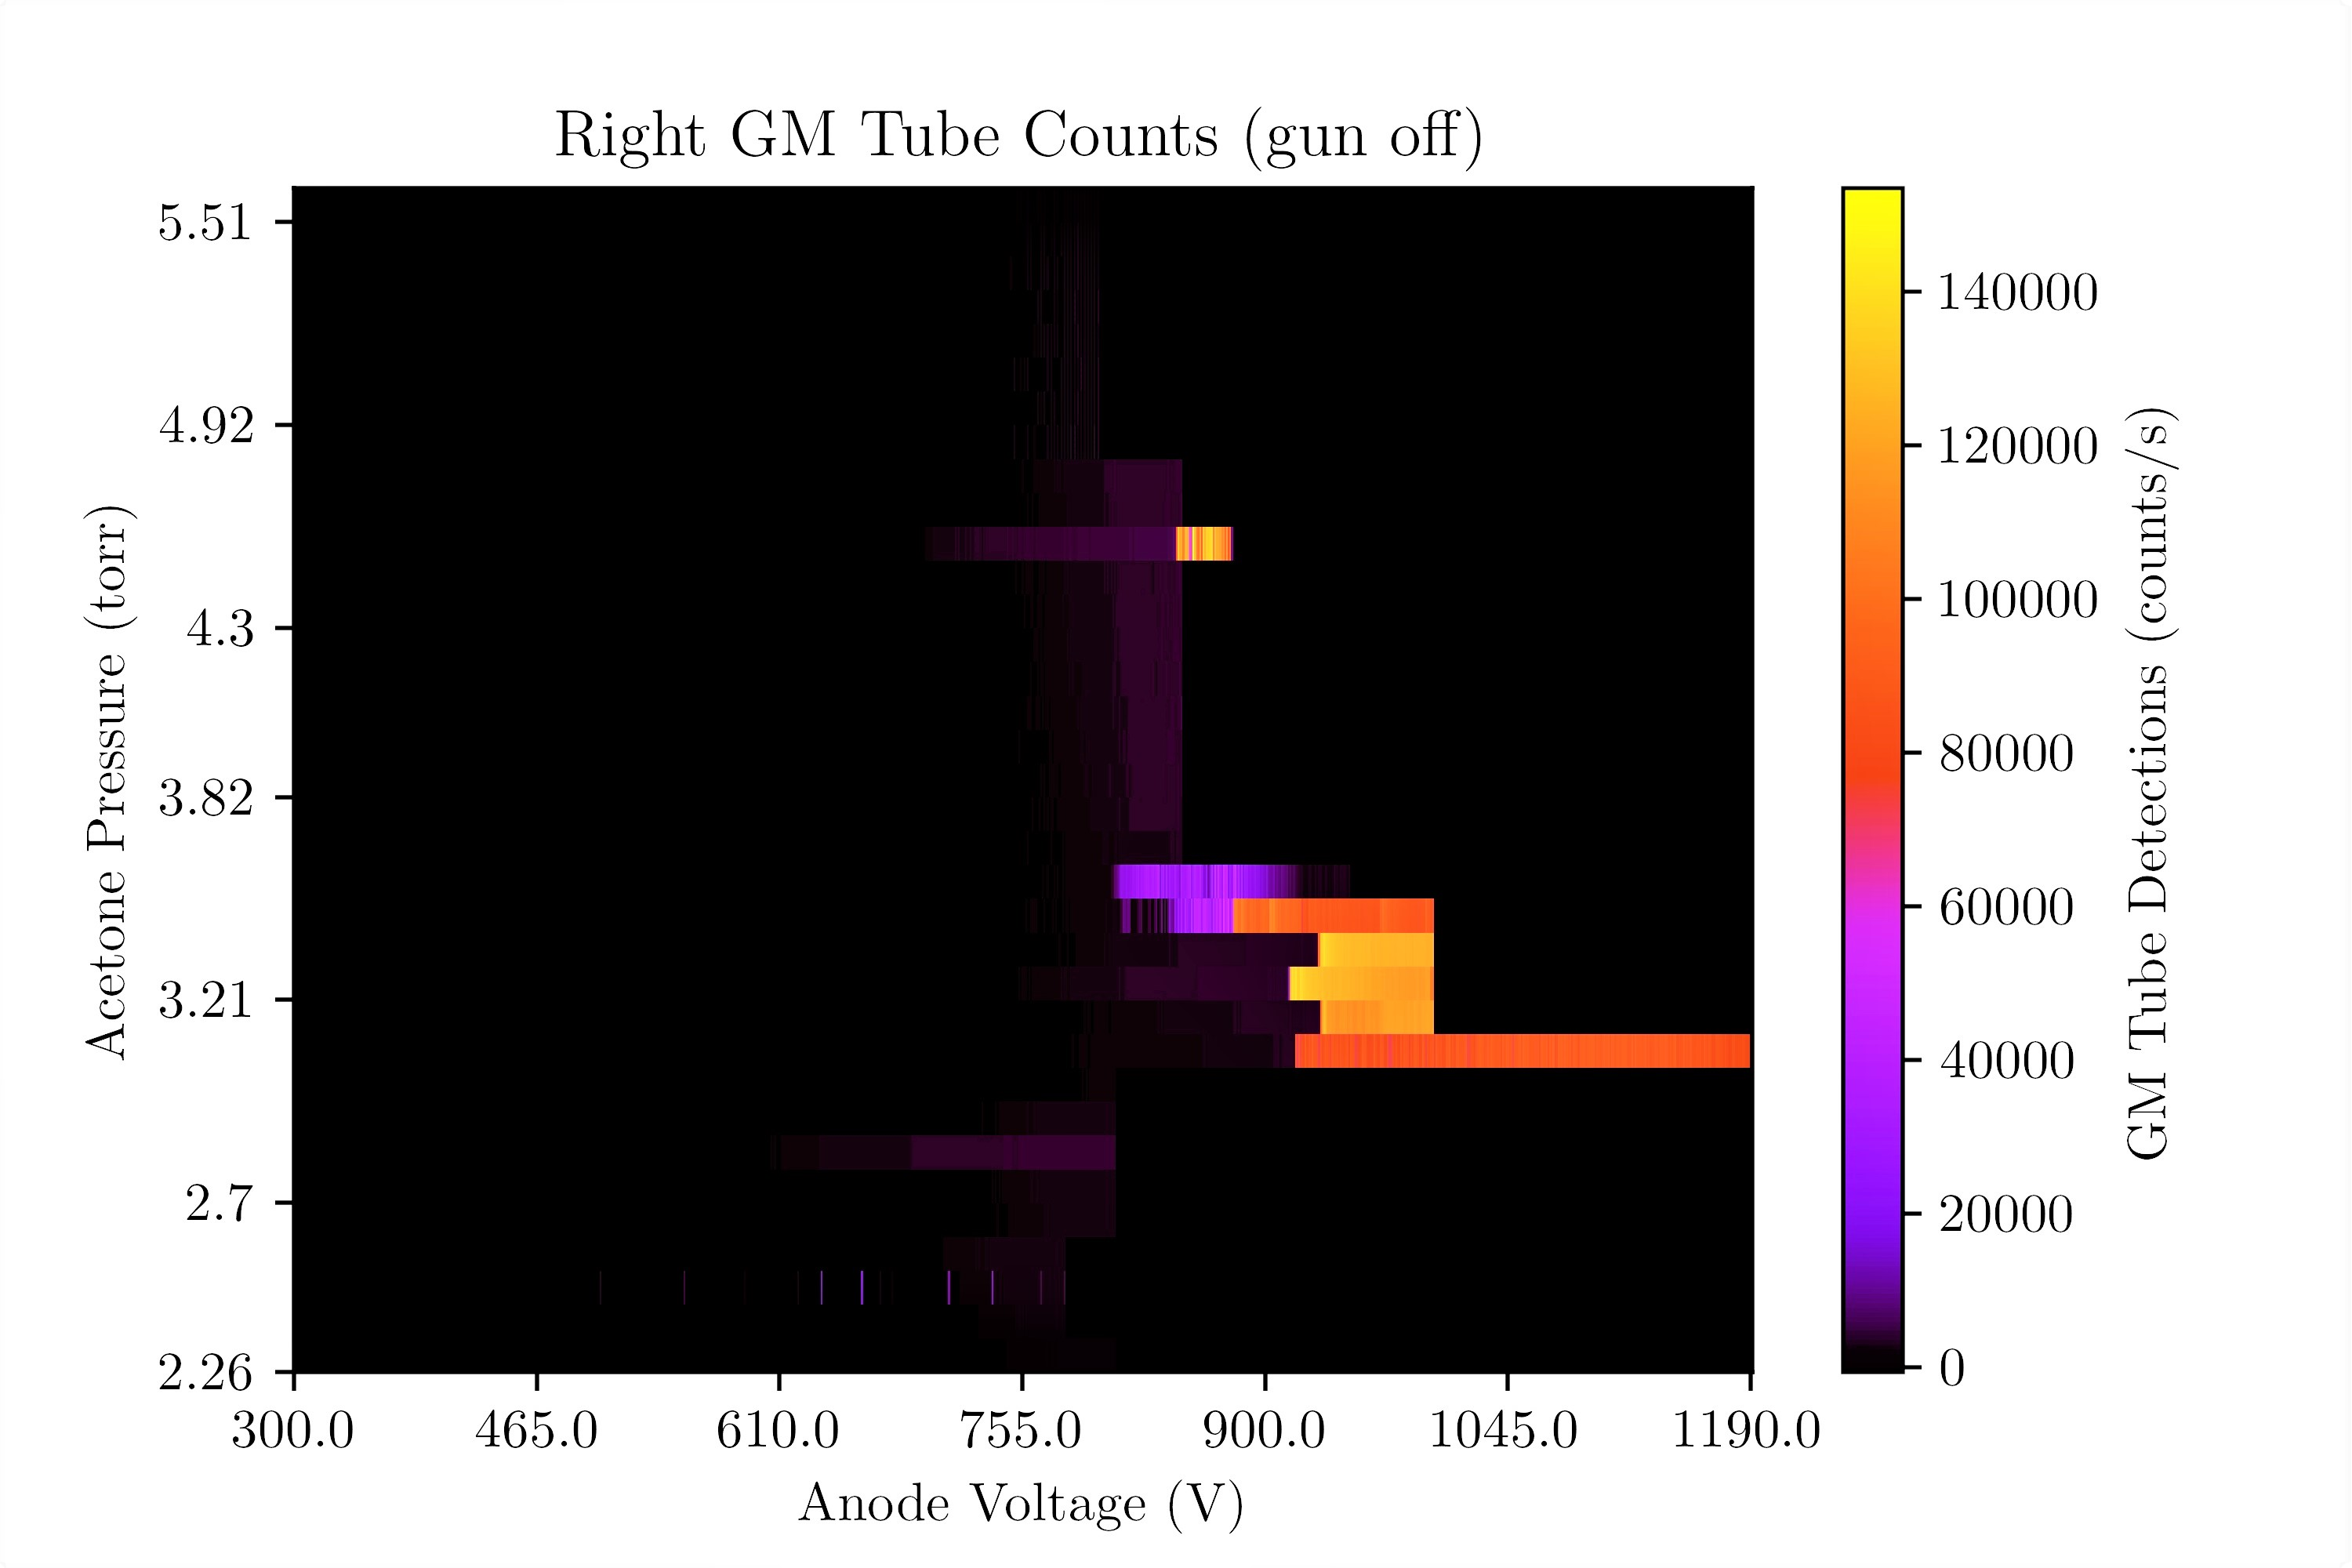
\includegraphics[scale=0.65]{Figs/RGMGunOff.jpg}}
    \subcaptionbox{Count rate from right GM tube as a function of anode voltage and acetone pressure. Electron gun on}[0.49\linewidth]{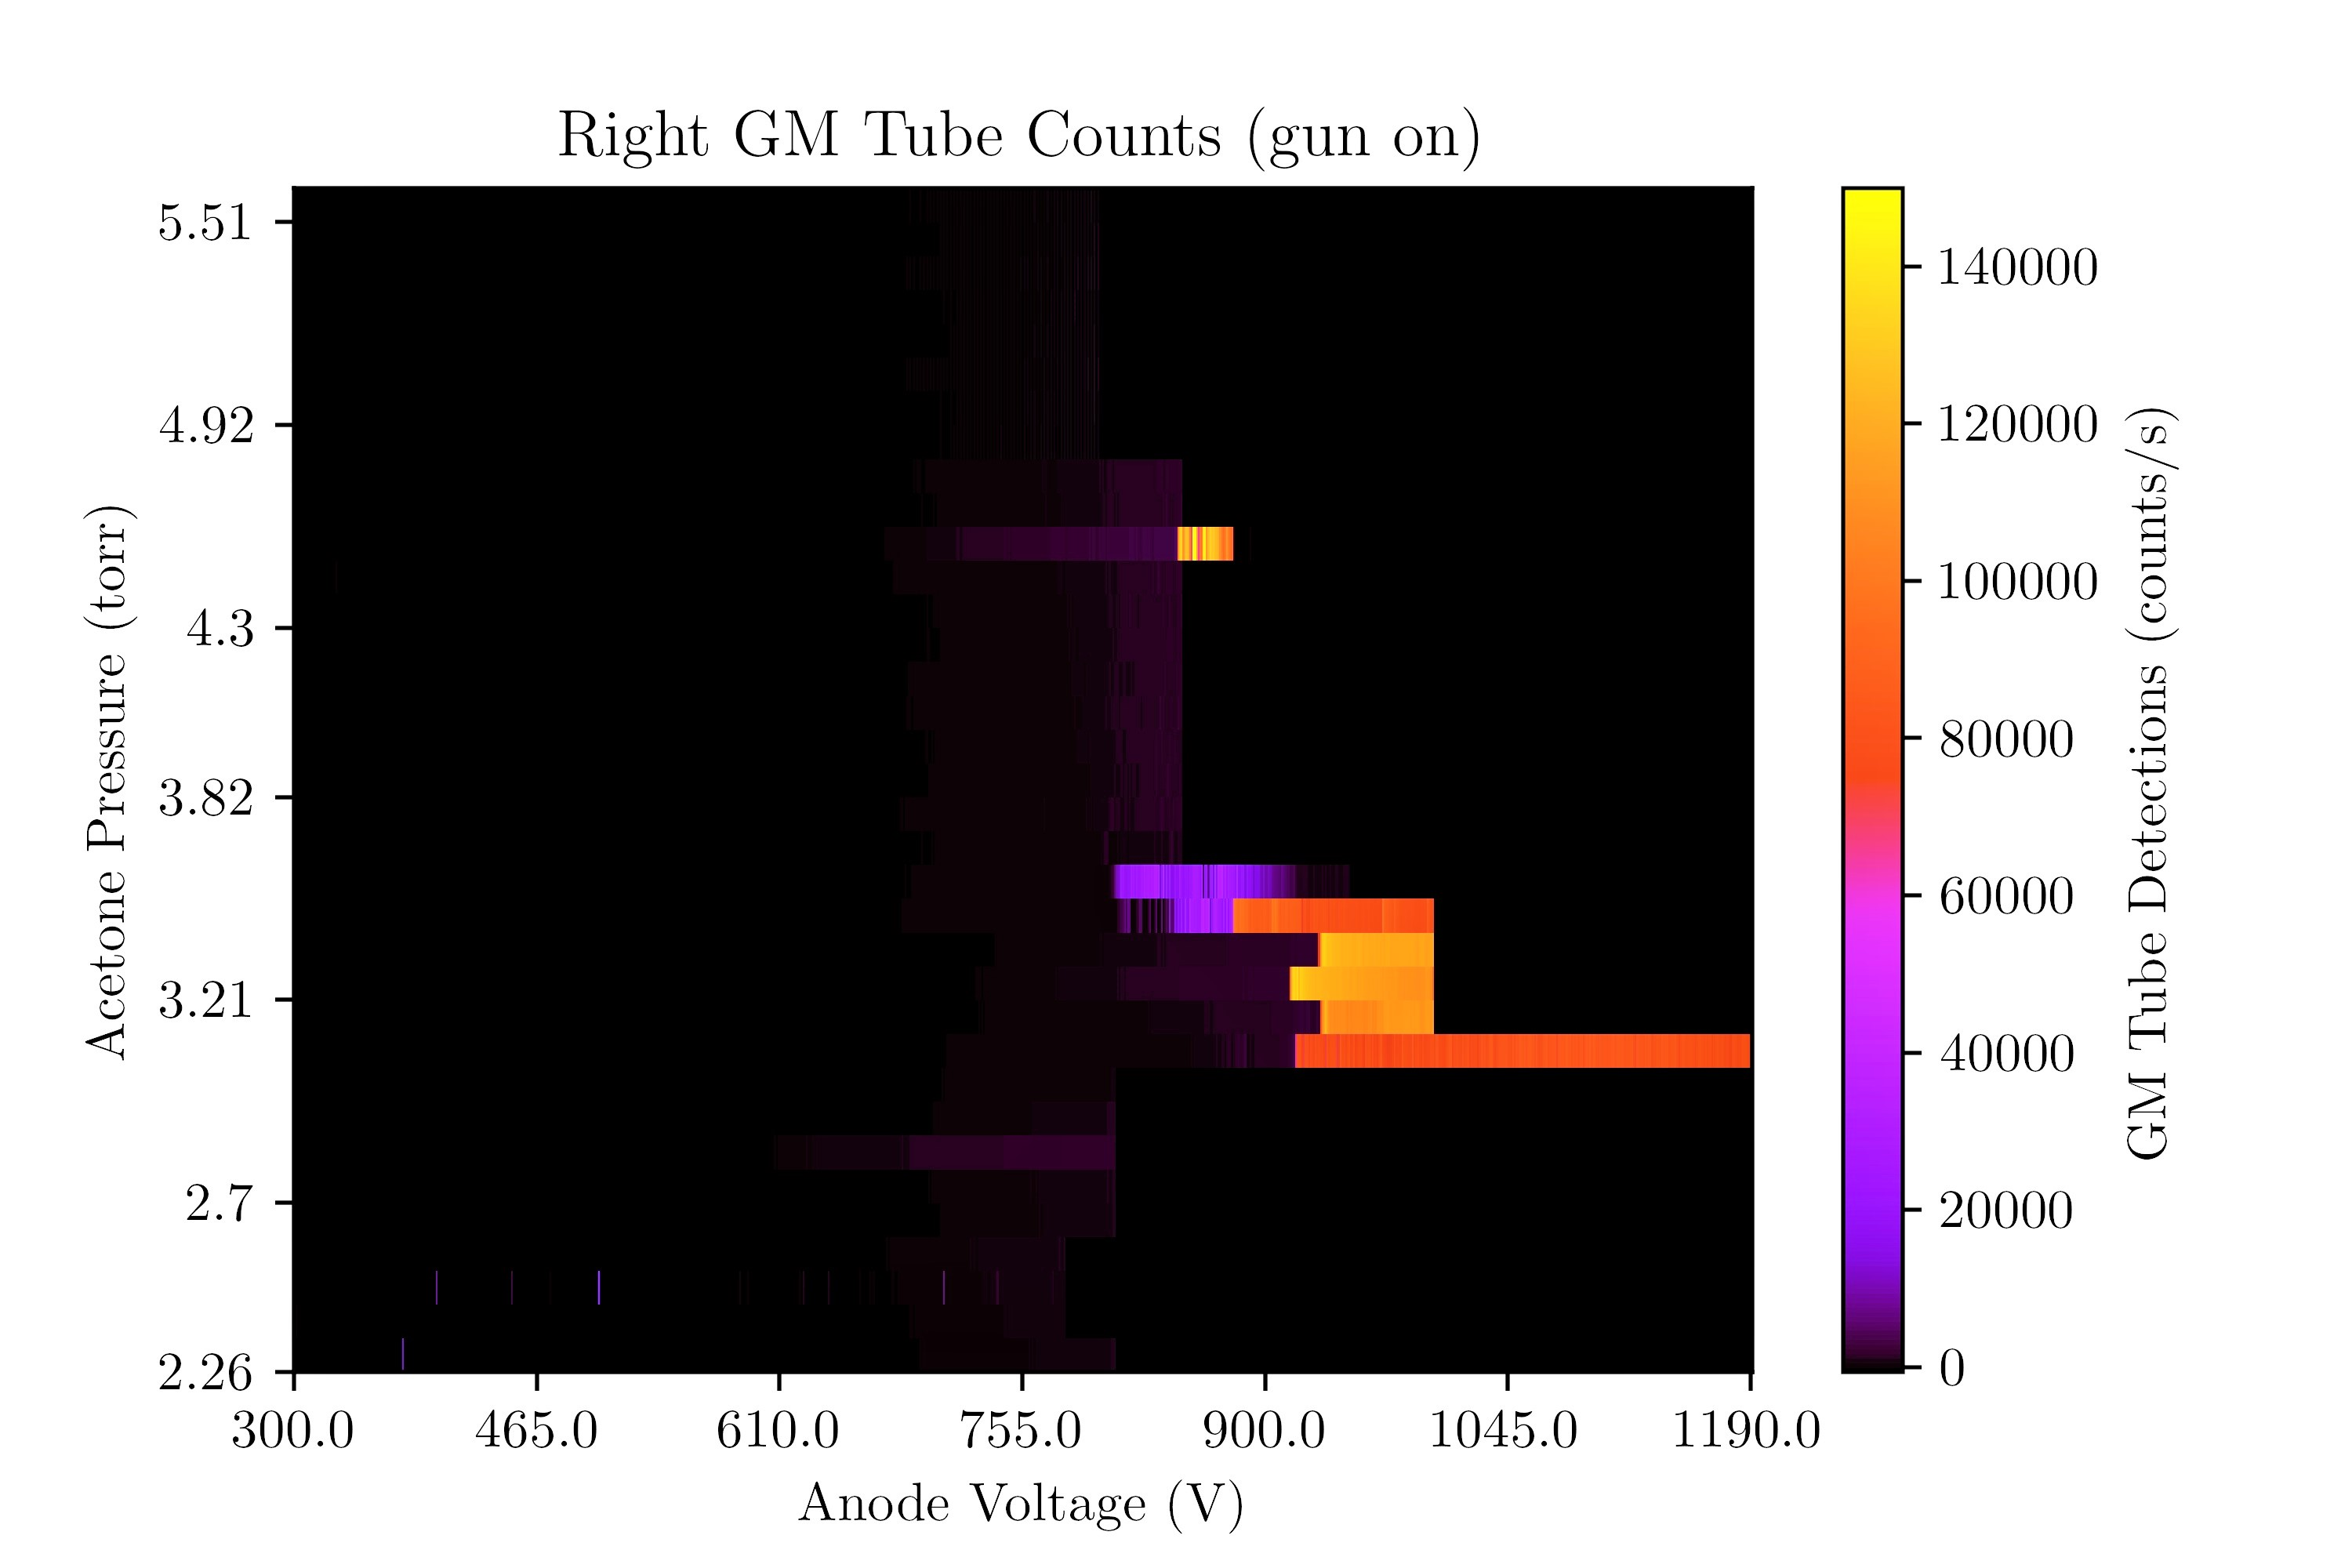
\includegraphics[scale=0.65]{Figs/RGMGunOn.jpg}}
    \caption{Performance of right GM tube over entire parameter space of pressures and voltages}
    \label{fig:paramRGM}
\end{figure}

For both tubes we see that there is an onset of counts earlier with the electron gun on than when the gun is off, these are indicative of detections of photons from the IPE of the copper sample.
By examining at what potential counts start to appear when the electron gun is off, we can determine the location of the breakdown voltage for each tube at each tested pressure. This 
gives us a new range of parameter space to explore, where the vast majority of counts can be attributed solely to IPE detections. The breakdown voltage was determined manually by examining plots 
of counts against anode voltage for each tube at each pressure. An example of such a plot can be found in \figref{VB}, and repeating for the remaining pressures yields \figref{breakdown}.

\begin{figure}[h!]
    \centering
    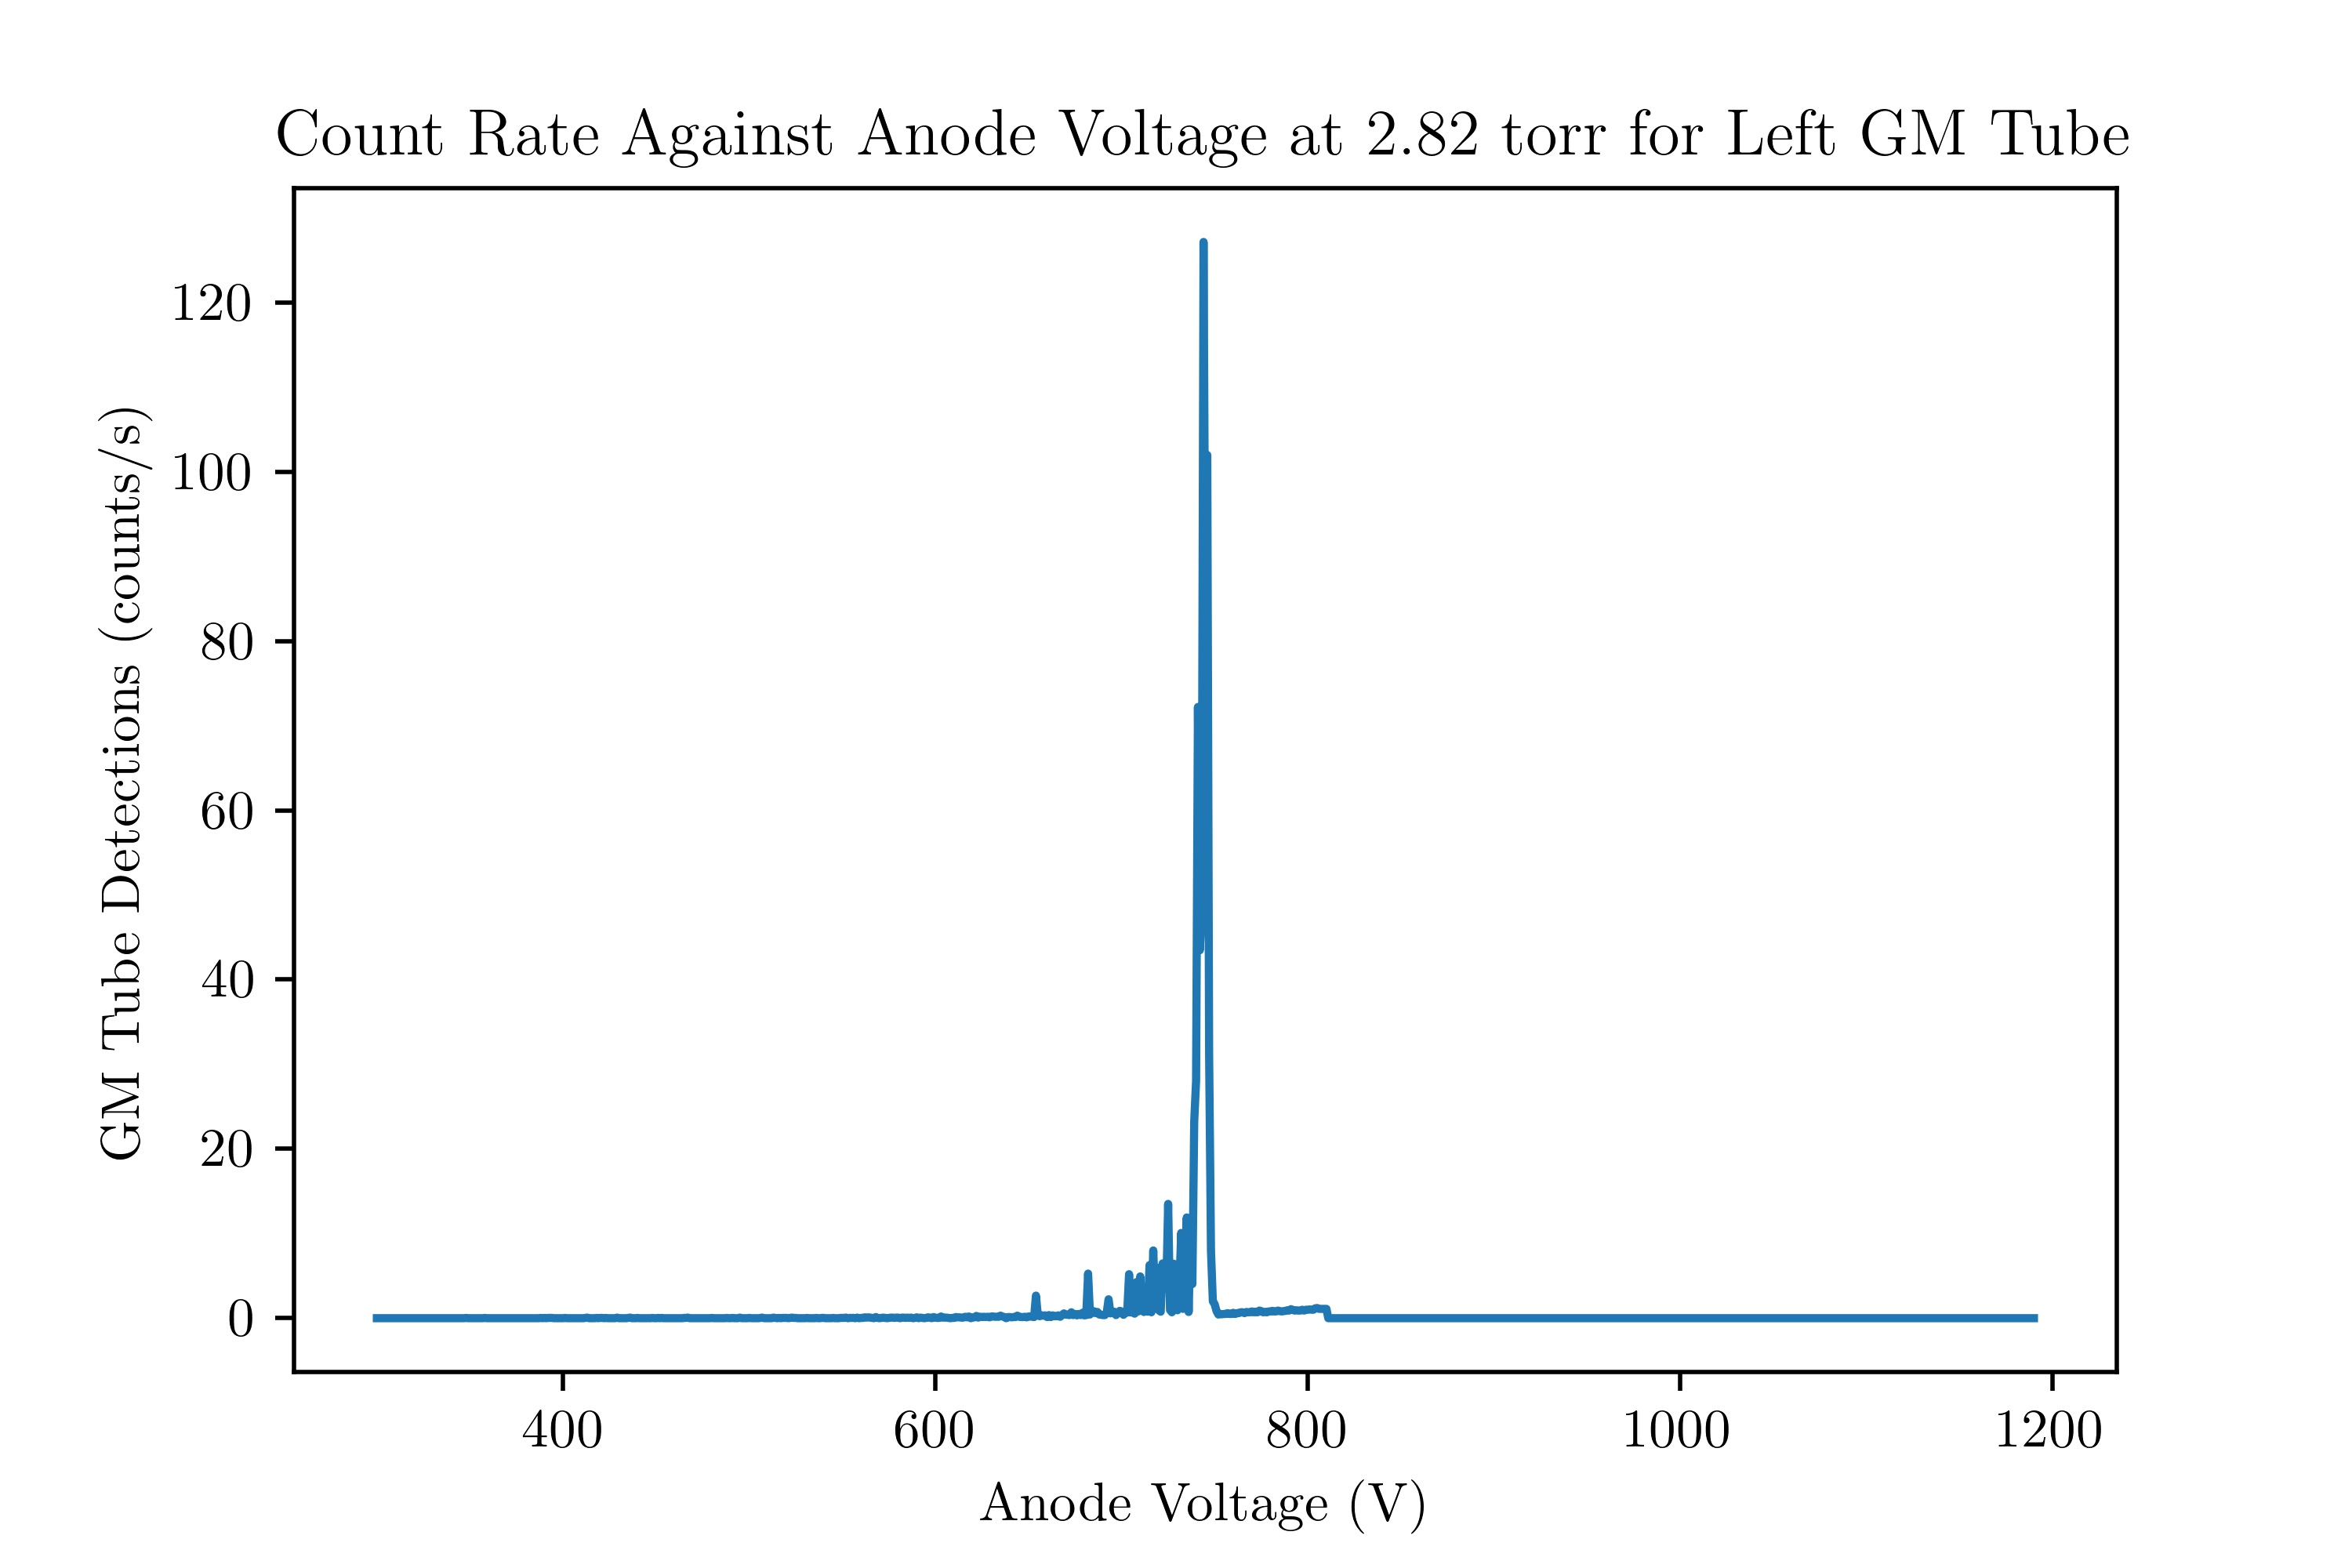
\includegraphics[scale=0.8]{Figs/example.jpg}
    \caption{Example of counts data as a function of voltage when electron gun is turned off. For this pressure, 2.82 torr, the breakdown voltage was determined to be 738V}
    \label{fig:VB}
\end{figure}

\begin{figure}[h!]
    \centering
    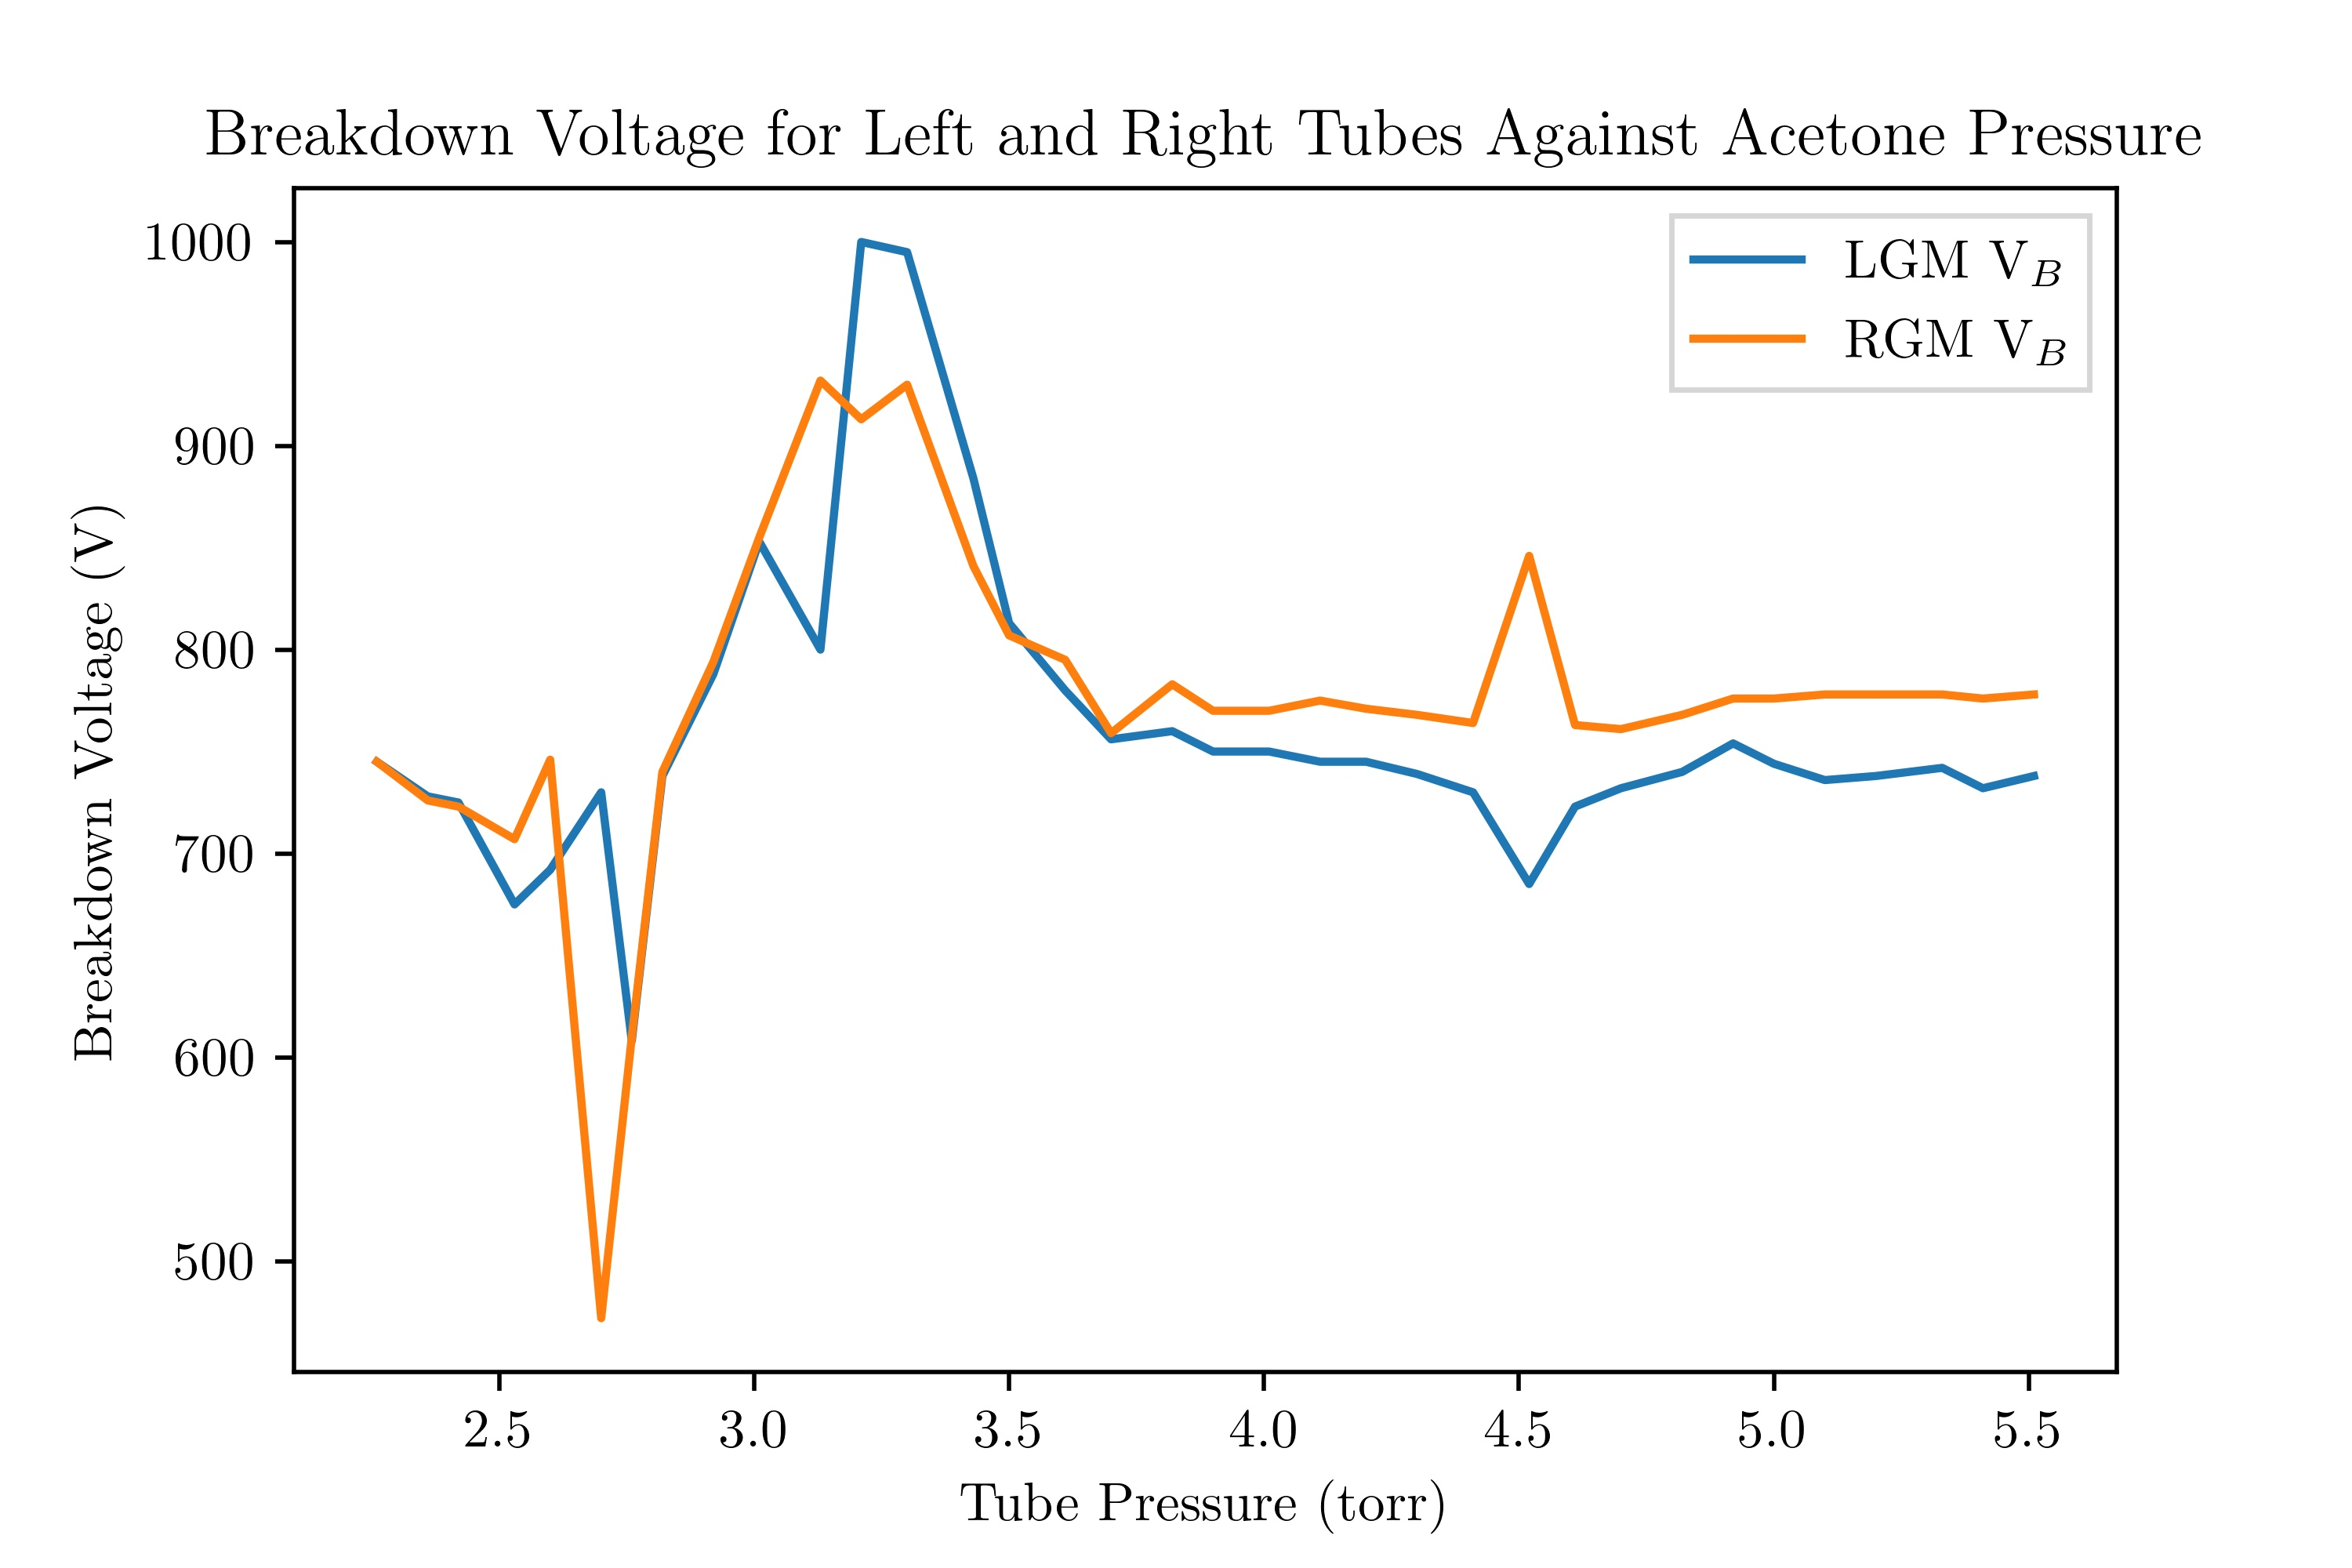
\includegraphics[scale=0.8]{Figs/VB.jpg}
    \caption{Breakdown voltages as a function of pressure for both left and right GM tubes}
    \label{fig:breakdown}
\end{figure}

With the breakdown voltages determined we can then truncate \figref{paramLGM} and \figref{paramRGM} to determine the regions of maximum counts and stability. A subtraction was 
also performed of counts while the gun is off from counts while the gun is on in order to provide a better estimate of the number of genuine detections at each configuration. 

\begin{figure}[h!]
    \centering
    \subcaptionbox{Counts for left GM tube below breakdown voltage}[0.49\linewidth]{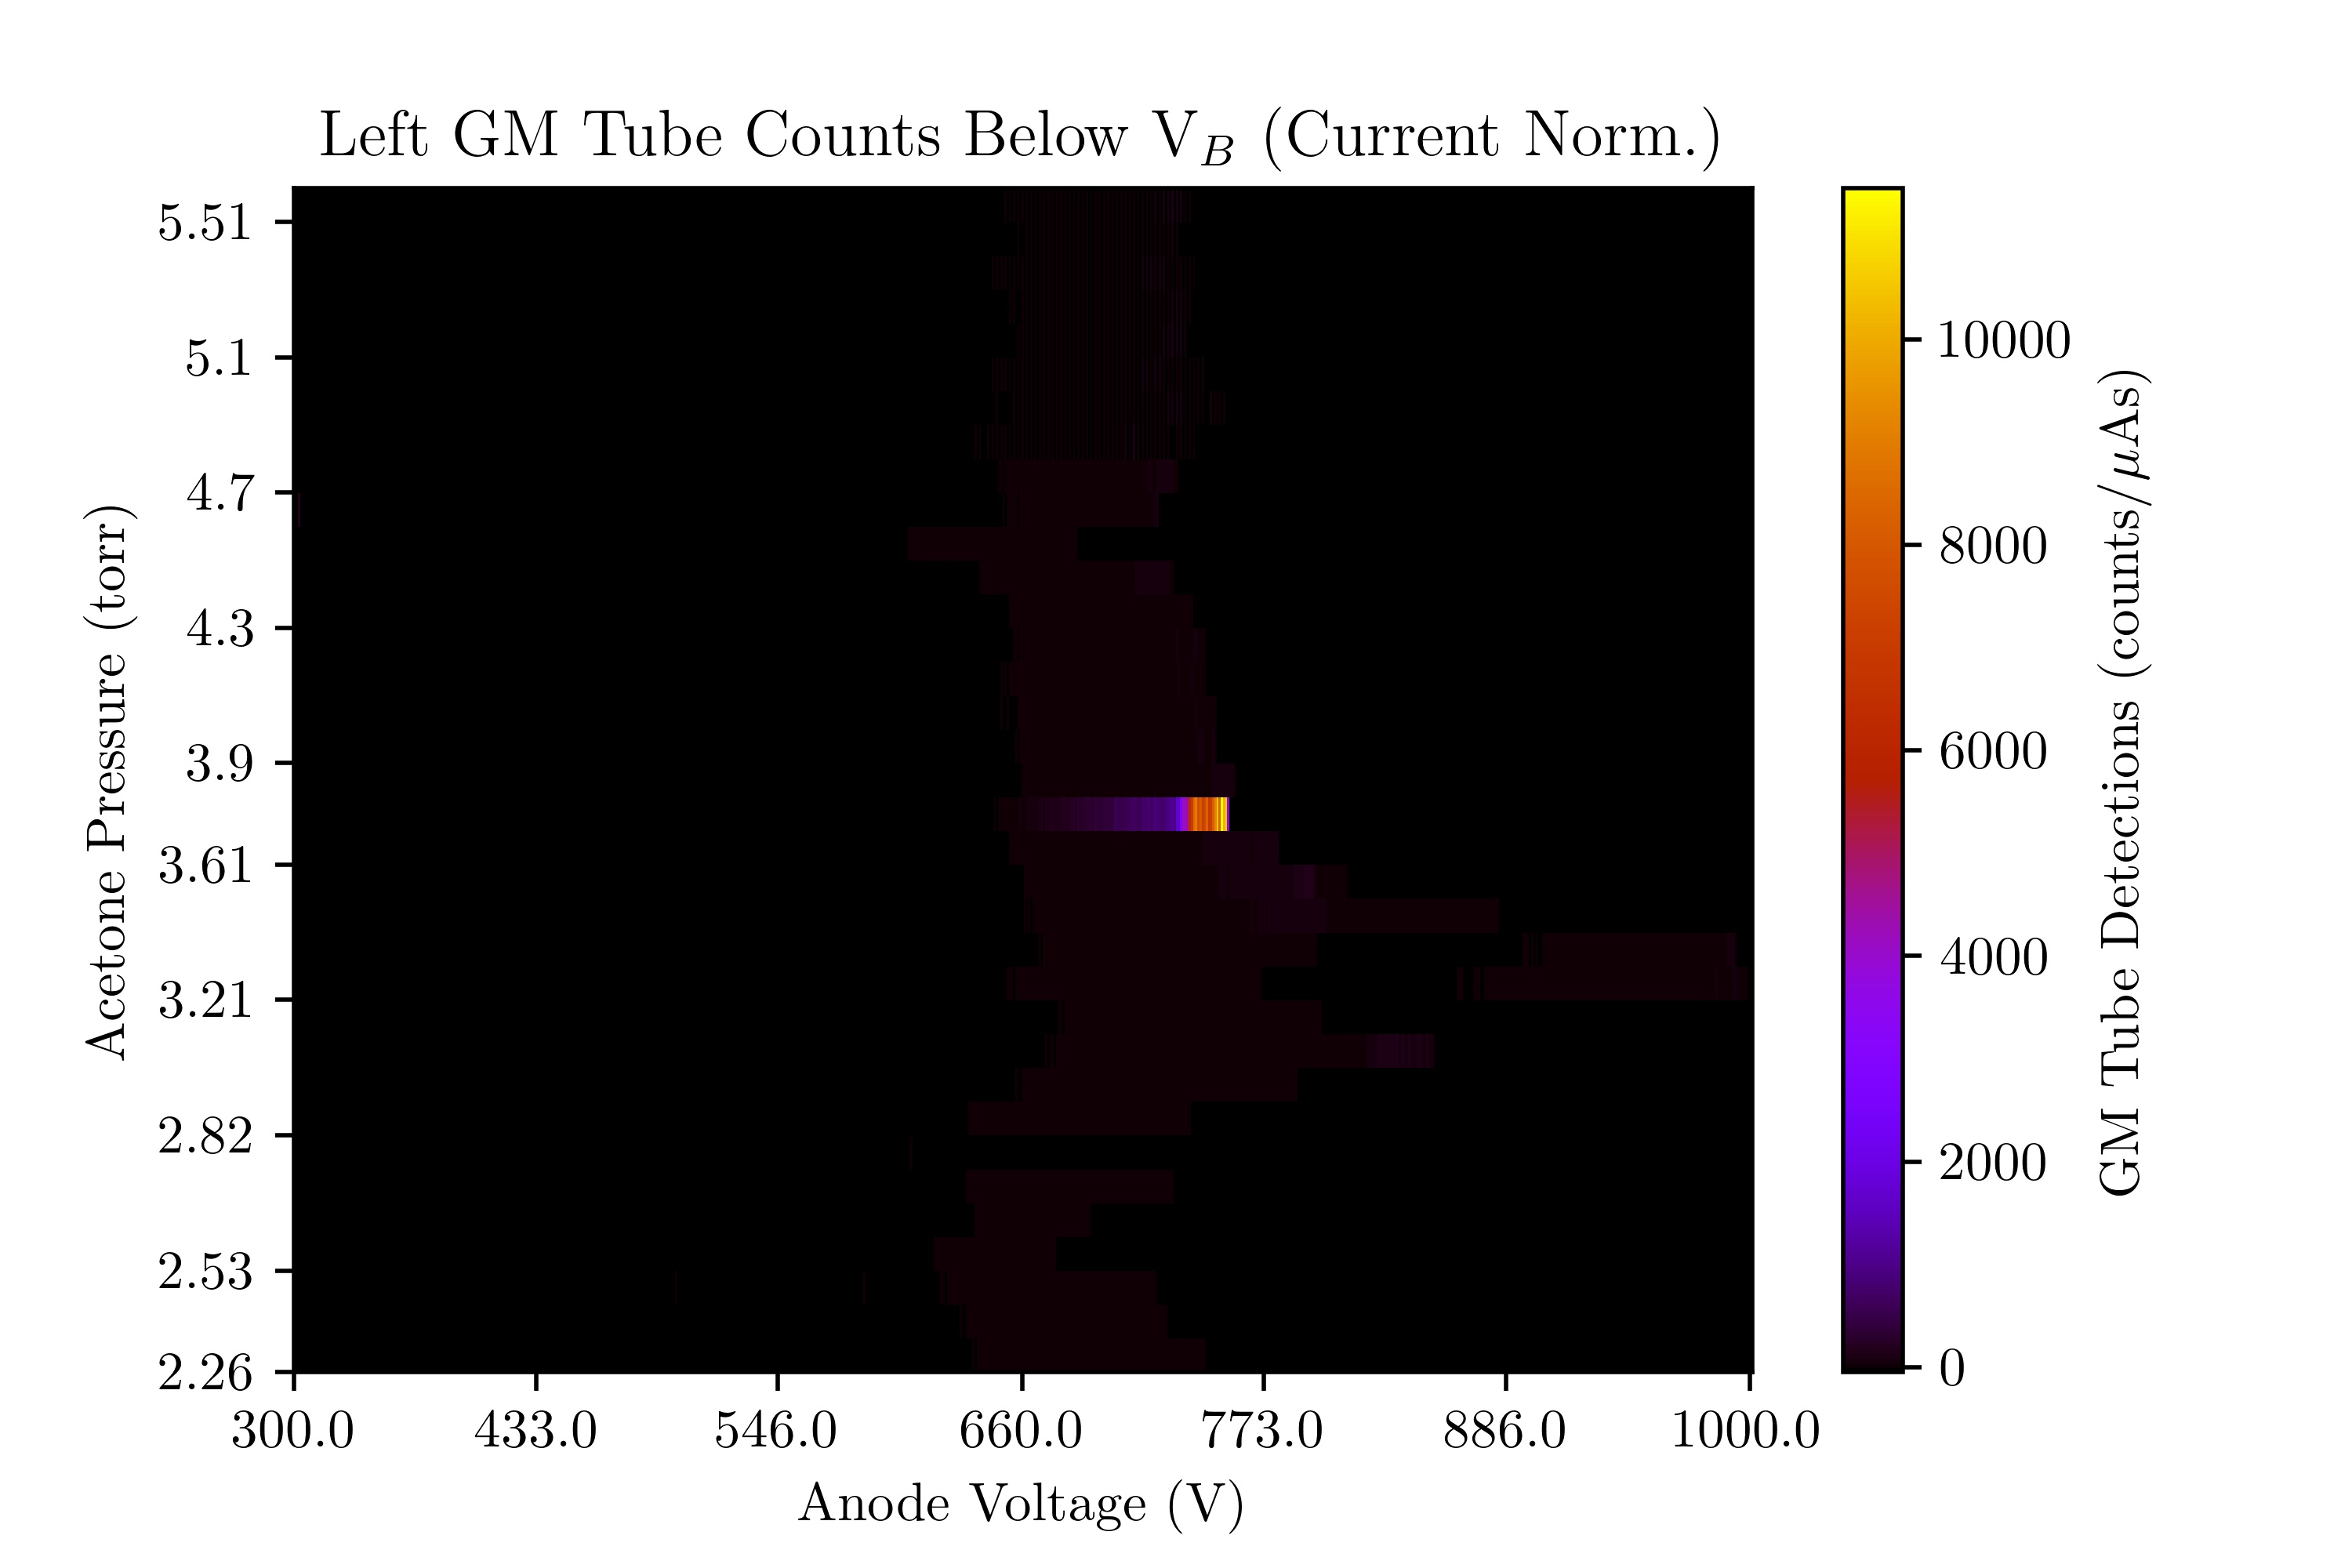
\includegraphics[scale=0.65]{Figs/LGMFinalNorm.jpg}}
    \subcaptionbox{Counts for right GM tube below breakdown voltage}[0.49\linewidth]{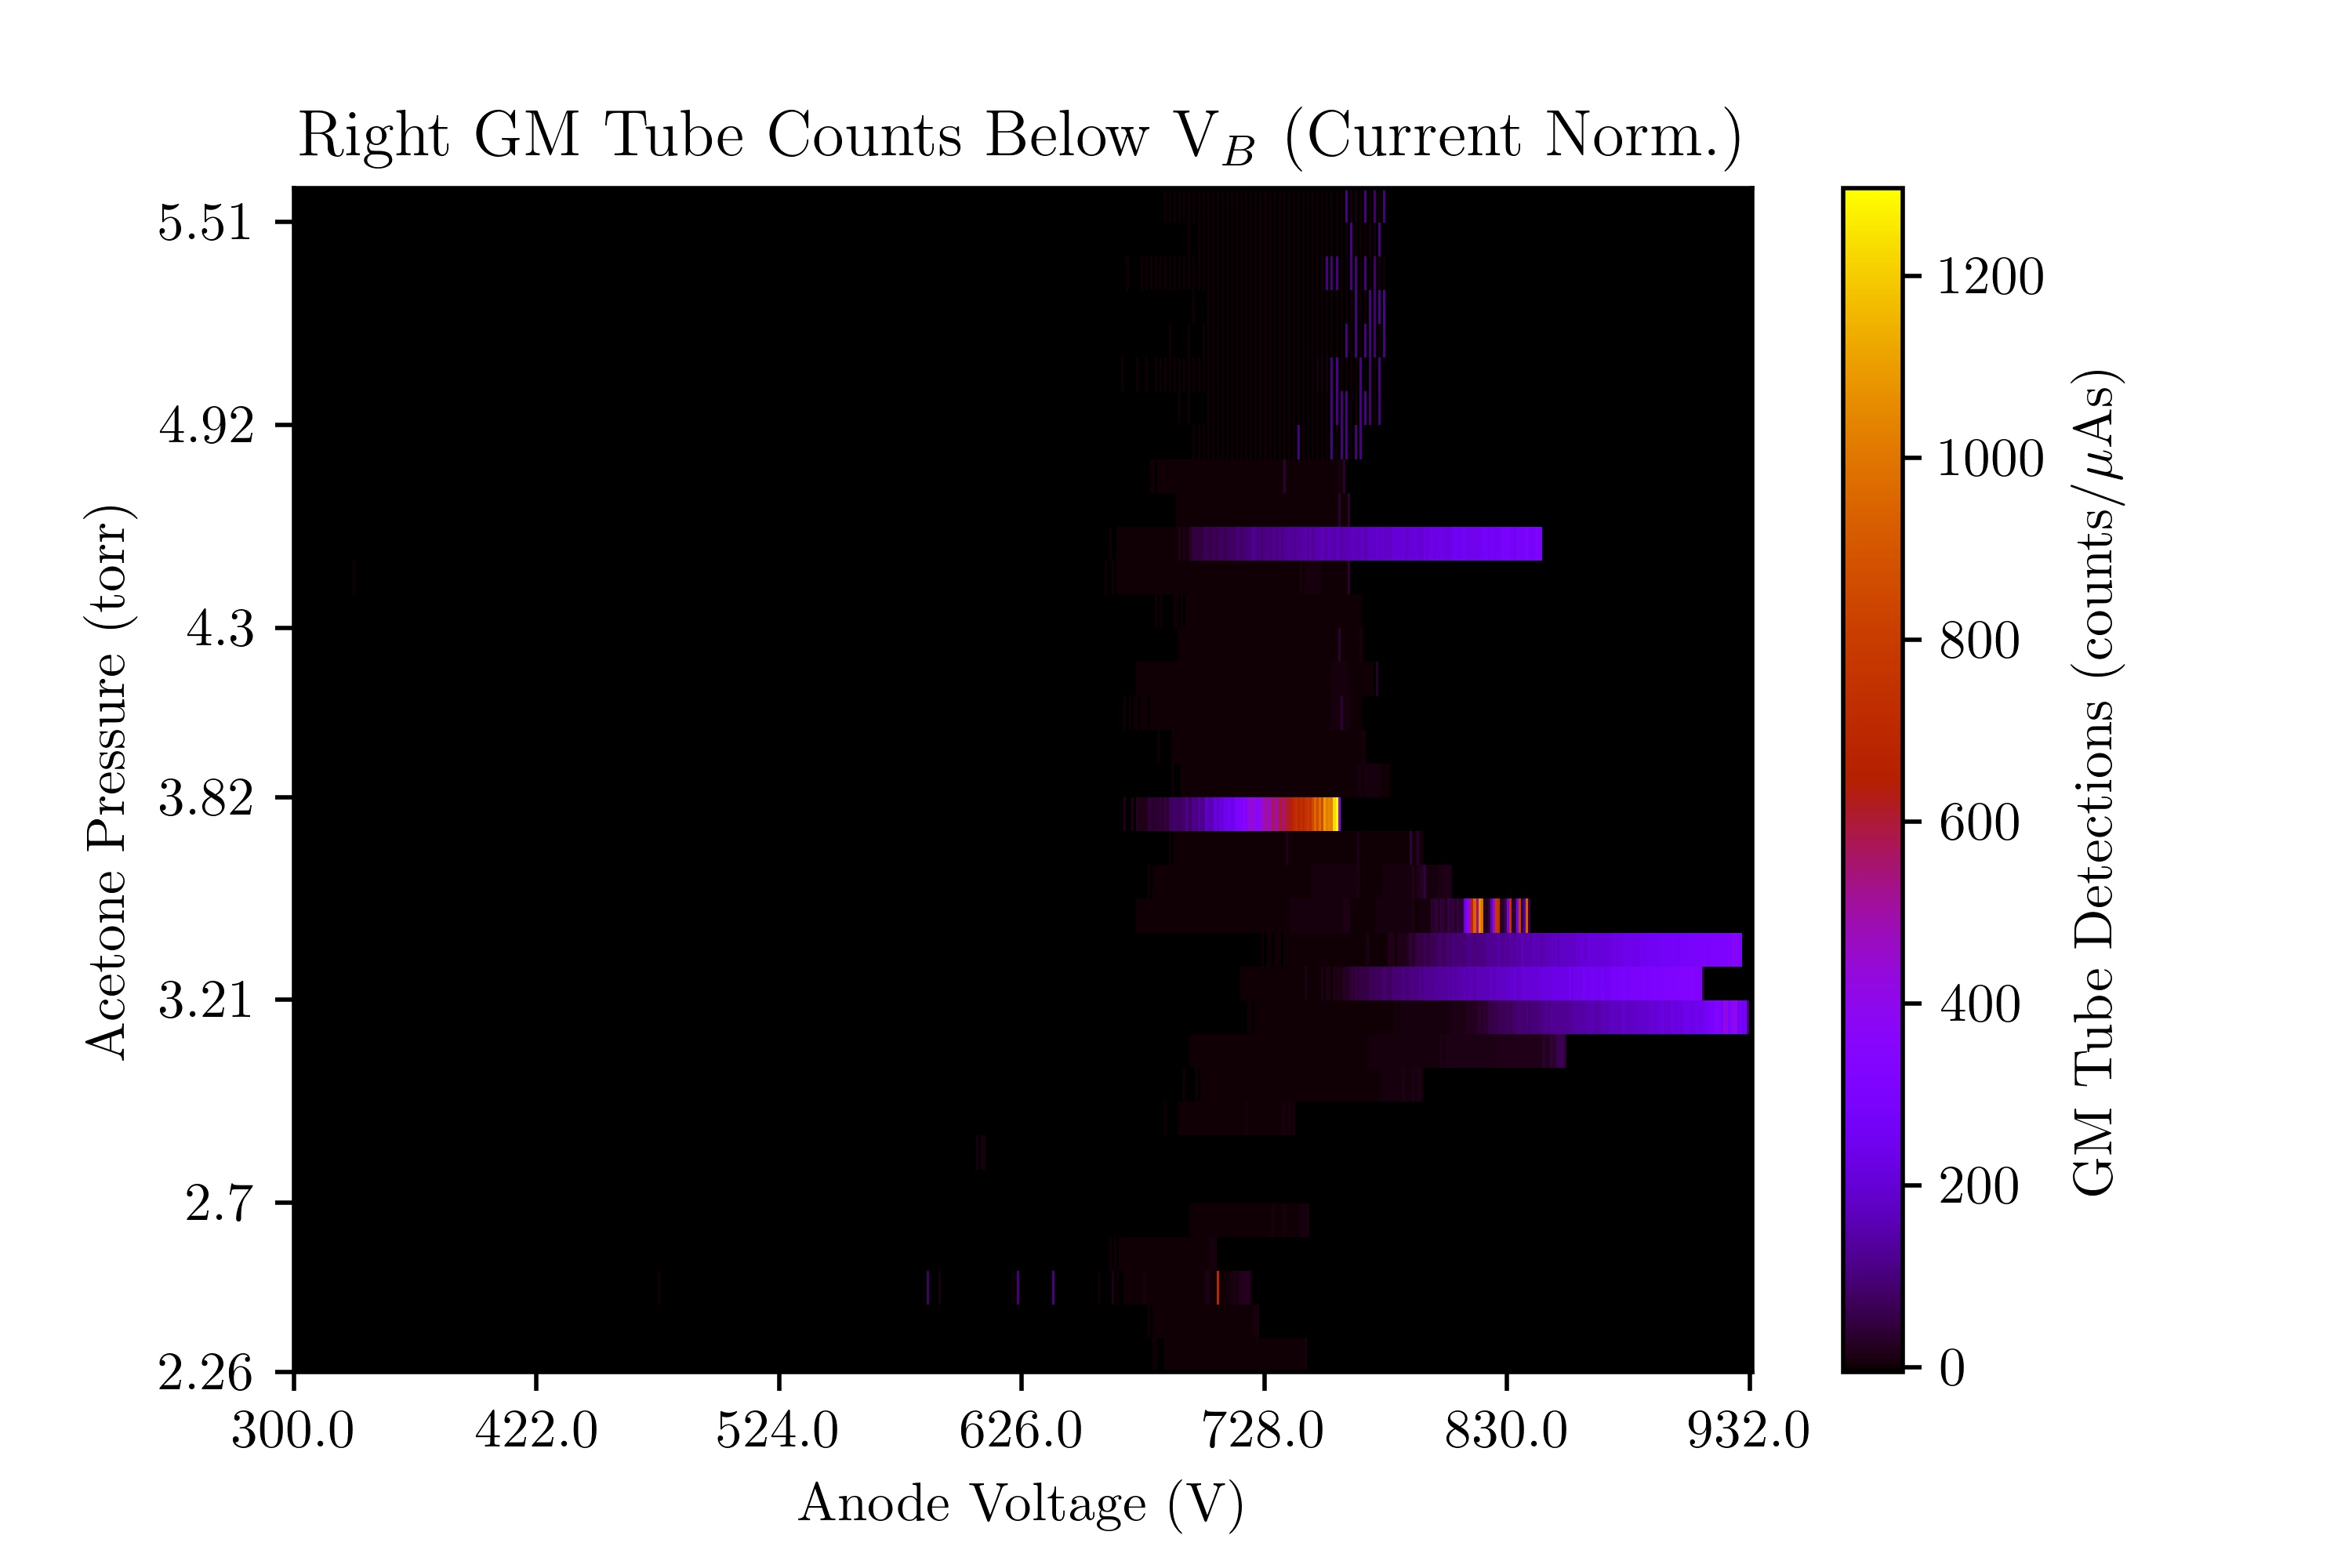
\includegraphics[scale=0.65]{Figs/RGMFinalNorm.jpg}}
    \caption{GM tube performance below breakdown voltage}
    \label{fig:results}
\end{figure}

Using this we determined optimal operating conditions for each tube to be:

\begin{table}[h!]
    \begin{center}
    \begin{tabular}{ccc}
    Tube & \multicolumn{1}{c}{\begin{tabular}[c]{@{}c@{}}Pressure\\ (torr)\end{tabular}} & \multicolumn{1}{c}{\begin{tabular}[c]{@{}c@{}}Anode Voltage\\ (V)\end{tabular}} \\ \hline
    Left & 3.70 & 740 \\
    Right & 3.70 & 750
    \end{tabular}
    \caption{Optimal conditions for left and right tubes }
    \label{tab:ideal}
    \end{center}    
\end{table}

We can consider a small subsection of these plots near the optimal region to see how the identified parameters compare to neighbouring regions. 

\begin{figure}[h!]
  \centering
  \subcaptionbox{Counts for left GM tube around identified optimal region}[0.49\linewidth]{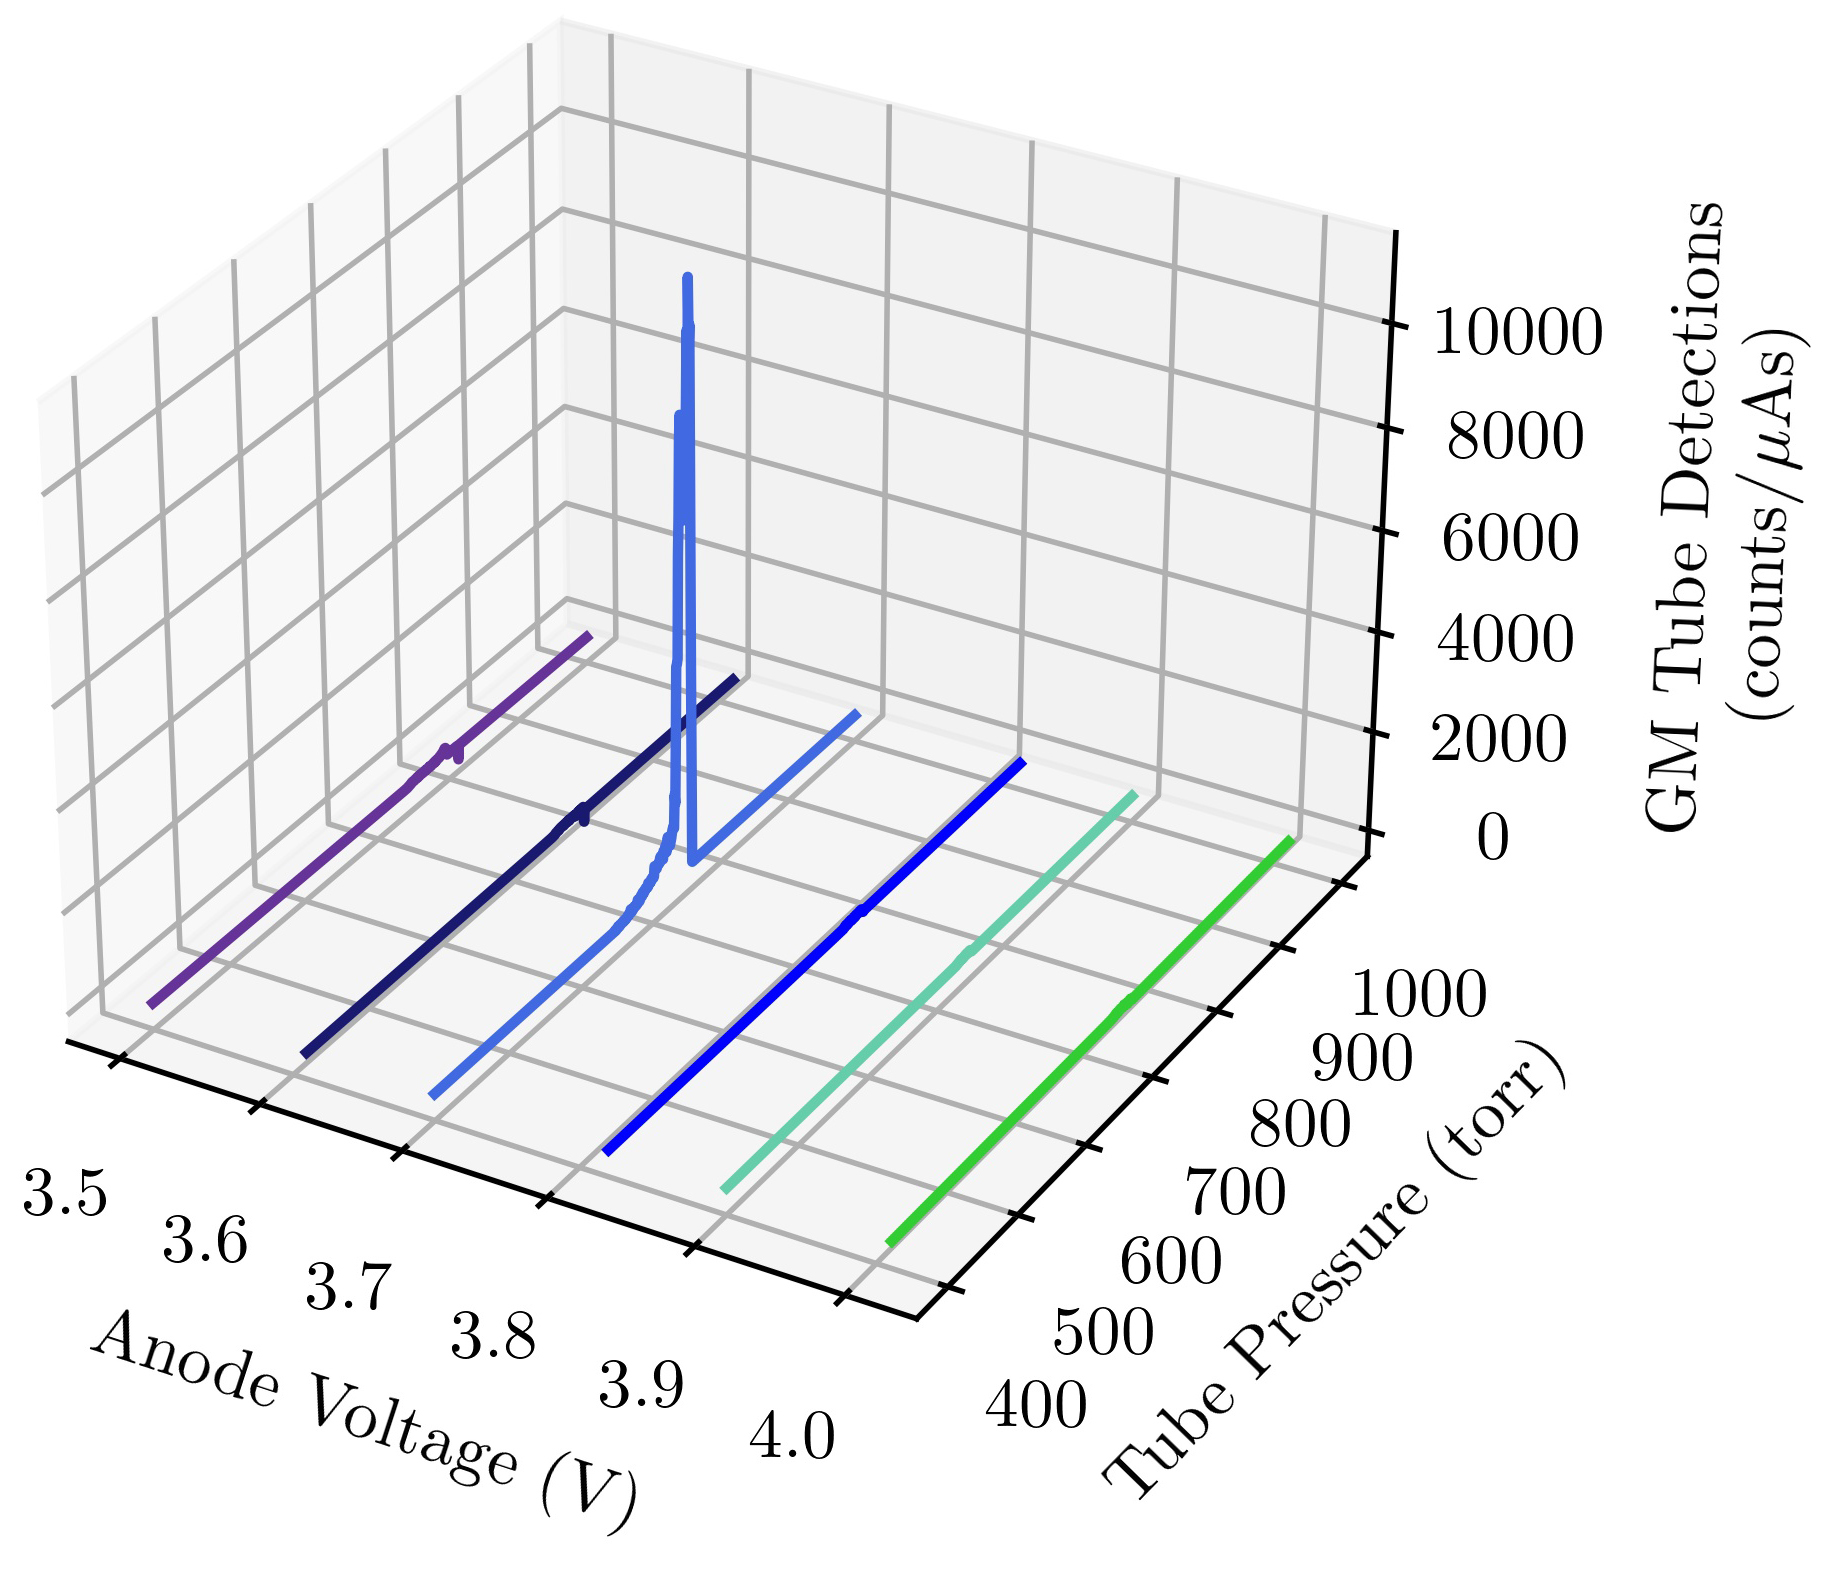
\includegraphics[scale=1]{Figs/LGM Waterfall.jpg}}
  \subcaptionbox{Counts for right GM tube around identified optimal region}[0.49\linewidth]{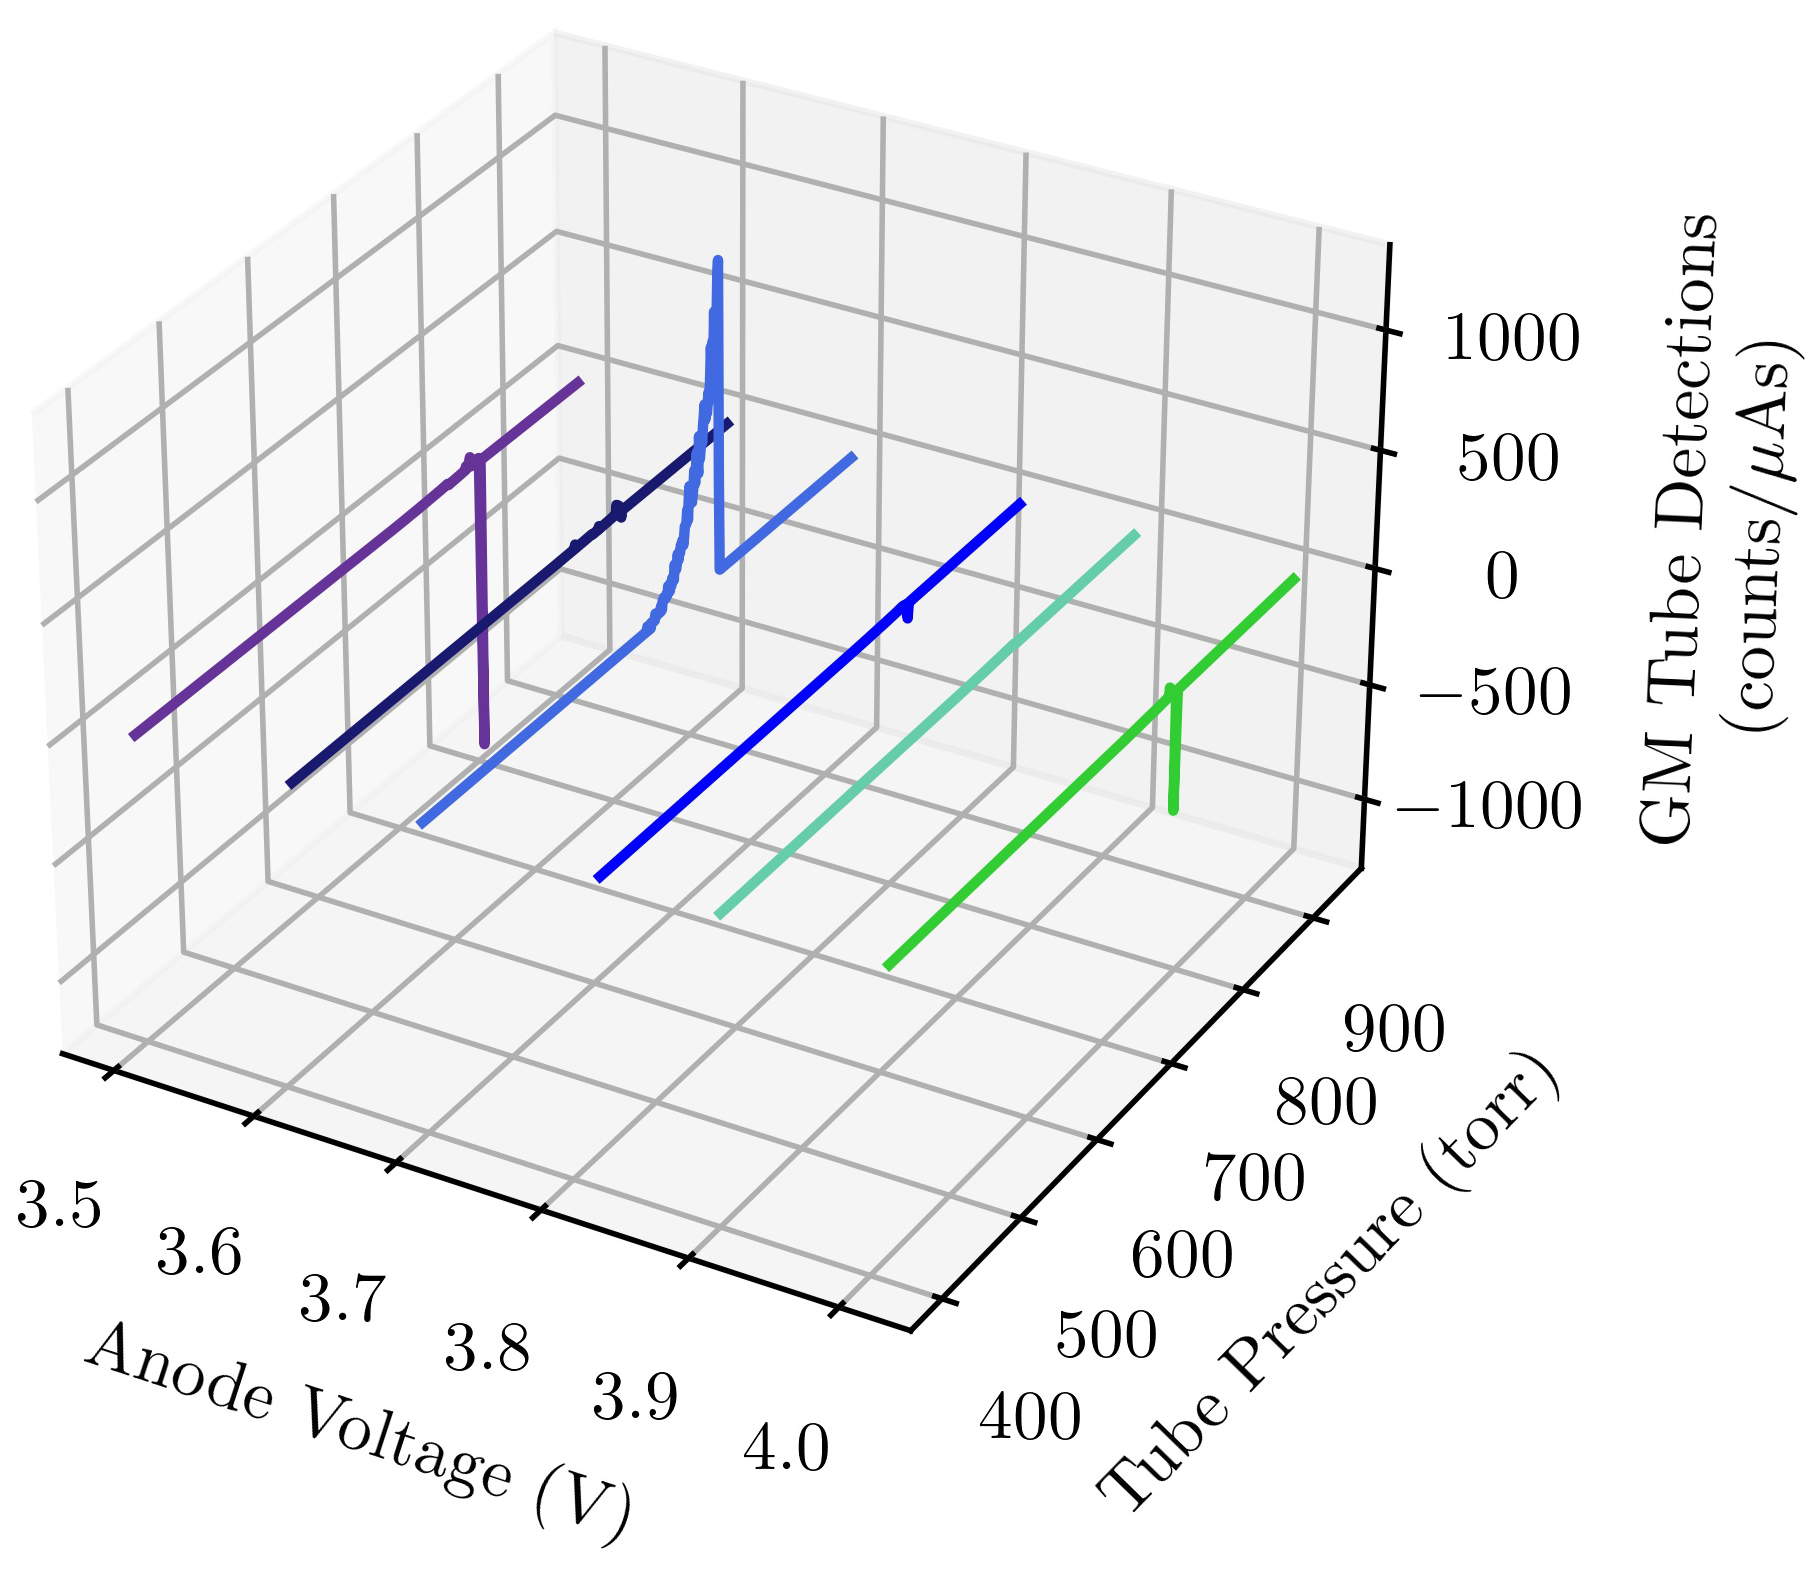
\includegraphics[scale=1]{Figs/RGM Waterfall.jpg}}
  \caption{Plots of counts for left and right GM tubes near their optimal operating conditions}
  \label{fig:waterfall}
\end{figure}

\section{Discussion}

Since the results are entirely dependent on determining the regions of parameter space which are stable (no tube breakdowns), we should begin by seeing if our result for breakdown 
match with what has been reported in literature. From the insert plot in \figref{litcompare}, we see that the results in our experiment match qualitatively with those obtained from Banik et al. early on, 
but diverge when our breakdown voltage reaches a maximum before decreasing and ultimately plateauing. While not explicitly stated in their paper, our tube's construction is almost certainly 
different from theirs, with the most important difference being the radius of the anode wire and inner diameter of the tubes. The most likely conclusion is that due to the geometry 
differences we are exploring more of the effects of tube breakdown over a similar pressure range. Since the tubes are completely independent systems once they are sealed from the 
gas manifold and have been designed to the same specifications, the fact that their breakdown voltages line up so strongly corroborates the notion that we are simply seeing more of 
the tubes' breakdown effects than Banik et al. 

\begin{figure}[h!]
  \centering
  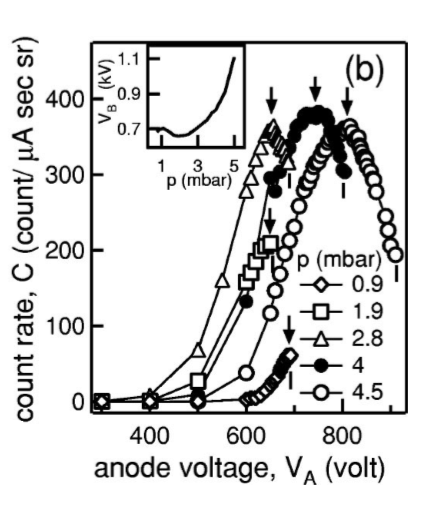
\includegraphics[scale=0.6]{Figs/litcompare.png}
  \caption{Main: Counts as a function of anode voltage for varying acetone pressure. Insert: Breakdown voltage as a function of pressure}
  \label{fig:litcompare}
\end{figure}

We see the maximal count rates for both tubes and how they compare to the rates of neighbouring regions in \figref{waterfall}. Though difficult to tell because of how much larger the 
results for 3.7 torr are (full size images available online), we see that each of the curves have the same shape: an initial large region of no detections, a sharp increase in 
count rate, then a maximum value before a sharp decrease after the breakdown is reached. This is exactly what we see in \figref{litcompare}, showing more qualitative agreement in how 
our GM tubes operate compared to what has already been published. 

In addition to the strong agreement in breakdown voltages for the two tubes, we see that they both achieve maximal count rates at 3.7 torr and within 10V of each other. We can use these
results to determine how the window material affects count rate. We know that the left tube uses \ce{MgF2} and the right tube uses \ce{CaF2}. The transmission threshold of \ce{MgF2} 
is reported to be 10.97eV\cite{lipton2002photon}, and 10.2eV for \ce{CaF2}\cite{funnemann198610}; further the photoionization potential of acetone is reported to be 9.7eV\cite{funnemann198610}.
This means we have a larger bandpass for the left tube than the right tube, i.e the right tube's window will absorb more photons than the left tube's and so we should expect less counts
from the right tube. Comparing the results shown in \figref{waterfall} we see that the left tube has a maximum count rate which is approximately 10 times larger than that of the right tube, 
which is exactly what we predicted based on the bandpass of the two detectors. Despite our desire for a high count rate, this is simply because IPES yields relatively few photons 
that we can detect; the energy resolution of the overall system is dependent only on the energy resolutions of the detectors and electron beams. These initial results however are 
not enough to make a determination on which window material we should use. While they show that the count rate with a smaller bandpass is still entirely useable for IPES, we need to 
consider the energy resolutions of both detectors in order to have a full picture on how one detector configuration compares to the other. This is commonly done in literature by 
performing IPES on a sample of polycrystalline gold or silver\cite{funnemann198610}\cite{maniraj2011high}, since their density of states is linear near the fermi energy. The resulting 
spectrum should be step function-like about $\varepsilon_F$ and the width of the function is indicative of the energy resolution. While this is an important experiment to perform in the coming term, it 
is important to note that it may have no impact on the detector setup since we may find that the current configuration is acceptable for obtaining accurate IPES results.

Obtaining pulse height distributions are another important component for understanding how the tubes operate, though we sadly ran out of time in the fall term before we could perform it.
The procedure involves simply filling the tubes to 3.7 torr, setting the appropriate anode voltages, and then letting the MCA run for long enough to obtain a statistically significant amount 
of detections. The pulse height data is automatically recorded by the MCA so we would simply need to fit an appropriate distribution to it and extract the mean pulse height and standard deviation. 
The mean pulse height (in volts), can be used in combination with the gain values of the electronics in order to determine the number of electrons involved in a given detection. A 
GM tube operating in the proportional count region will have detections involving on the order of $10^4$ electrons, whereas a detector operating in the geiger region will have 
detections involving on the order of $10^9$ electrons\cite{knoll2010radiation}. While both proportional and geiger regions are acceptable for IPES, the geiger region is less stable 
for the detector over a long period of time. This means needing to refresh the acetone more often than if the detector is operating in the proportional count region, and a greater 
risk to the electronics due to the larger current pulses. Therefore if we determine that at the parameters outlined in table \ref{tab:ideal} have the detectors operating in the 
geiger region we may need to consider a new region which has a lower count rate but is in the proportional count region and thus further from tube breakdown. 

\section{Conclusion}
We investigates the photodetection capabilities of two gas filled bandpass detectors for use in inverse photoemission spectroscopy. Maximum count rates were found at an acetone 
pressure of 3.7 torr and an anode voltage of 750V for the tube with a \ce{CaF2} entrance window, and 3.7 torr at 740V for the tube with a \ce{MgF2} entrance window. We further determined
that due to the smaller bandpass of the \ce{CaF2}, the count rate obtained at this optimal operating was significantly smaller than the tube with a \ce{MgF2} entrance window with a 
larger energy bandpass. Due to time constraints we were unable to determine the energy resolution of the tubes at these operating conditions, though we proposed a method to do so 
in the new term which involves performing IPES on polycrystalline gold or silver and looking at the broadening near the fermi energy. We were also unable to examine the pulse height 
distributions of the two tubes, which can be used to find an average pulse height, and thus determine the operating region of the tubes based on the number of electrons in each detection. 

We have also shown that the two tubes, which are completely isolated systems and constructed to identical specifications, showed strong agreement in what parameters yielded the most 
counts and at what voltages breakdown would occur. These results also agreed qualitatively with those reported by Banik et al., whose experiment inspired the work done for this report. 
This leads us to conclude that we have successfully examined the relevant ares of parameter space for our tubes, their breakdown voltages, and thus the optimal conditions at which we should 
be operating. 

Building on these results in the next term, we hope to finish our analysis of the GM tube performance and then shift focus to optimizing the performance of the electron gun set up. 
The parameter space of the gun is much larger than the tubes, and extracting relevant information like beam width is a complicated procedure so we hope that the remaining work on the GM 
tubes can be completed very quickly. We also hope to finally obtain good IPES spectra from various samples kept in the lab which agree with those reported in literature. Most important 
among these being polycrystalline gold and silver, a full scan of Cu(111), and the image-potential states of Cu(100).

\clearpage
\section{Acknowledgements}
I'd like to thank my supervisor, Prof. David Hawthorn, for providing me the opportunity to learn and grow as a researcher. I've been working with him for 8 months now and have learned
so much about condensed matter physics, experimental skills, and how to think like a physicist. I'd also like to thank all of the members of the Hawthorn group, who were always there 
to offer advice when I got stuck, celebrated my successes, and shared the amazing projects they're all working on. Finally thank you to those of you who dedicated your time to read 
my report, I appreciate your efforts greatly. 
\clearpage